\documentclass{fulbrightthesis}
\usepackage{marktext}
%% 14pt font size — using fontsize package (no blank page side effects)
\usepackage[fontsize=12pt]{fontsize}

\usepackage{fuvmacro}
%% all the packages should go to fuvmacro PLEASE ADD AS NEEDED AS LONG AS IT DOES NOT INTERFERE WITH EXISTING FORMATTING

%% Additional packages needed for thesis content
\usepackage{float}
\usepackage{booktabs}
\usepackage{caption}
\usepackage{longtable}
\usepackage{tikz}
\usetikzlibrary{arrows.meta, positioning}
\usepackage{pgfplots}
\pgfplotsset{compat=1.18}
\usepackage{setspace}
\graphicspath{{figures/}}

%% Title — matches template title page format exactly
\title{Renewable Intermittency and Grid Investment Dynamics: The Role of Scarcity-Induced Battery Innovation in Vietnam}

\author{Name: Toan T. Nguyen \\ Advisor: Dr.\ Xavier Martin G.\ Bautista}

\degree{Bachelor of Arts in Economics}
\degreedate{Spring 2025}

%end the preamble and start the document
\begin{document}
\baselineskip=18pt plus1pt
\setcounter{secnumdepth}{3}
\setcounter{tocdepth}{3}
\maketitle

%% ---------------------------------------------------------------
%% DEDICATION PAGE (no page number)
%% ---------------------------------------------------------------
\begin{dedication}
    To all who made this possible.
\end{dedication}

%% ---------------------------------------------------------------
%% ROMAN-NUMBERED FRONT MATTER
%% Order from template PDF:
%%   TOC (i) to Abstract (ii) to Acknowledgements to List of Tables to List of Figures (v)
%% ---------------------------------------------------------------
\begin{romanpages}

\tableofcontents

\clearpage
\section*{Abstract}
\addcontentsline{toc}{section}{Abstract}
I investigate the divergence between rapid private renewable deployment and slow public grid investment which is known in engineering as the ``agility gap.'' I develop an open-economy DSGE model with endogenous scarcity-induced technological change in battery storage and a grid reliability constraint, where variable renewable penetration creates intermittency shocks that reduce capital utilization through grid instability. 

Calibrating the model to Vietnam's Power Development Plan 8, I find the following. First, the agility gap is quantitatively large and structurally asymmetric: battery investment responds quickly to reliability shortfalls but is governed almost entirely by global price shocks (100\% of its variance), while grid investment responds to domestic reliability signals but accumulates slowly through the fiscal rule (82\% of its variance). The two flexibility instruments are therefore driven by entirely separate forcing variables, international supply chains versus domestic fiscal decisions, which is why private storage deployment and public grid expansion cannot be treated as substitutes in policy design. Second, scarcity-induced technological change generates persistent battery improvements conditional on regulatory transmission of scarcity signals. Third, suppressing scarcity signals raises the welfare cost of intermittency by 20\%, demonstrating that market mechanisms are quantitatively important complements to storage investment.

\vspace{0.5cm}
\noindent \textbf{Keywords:} Environmental DSGE, Scarcity-Induced Innovation, Endogenous Technological Change, Investment Inertia, Renewable Intermittency, Energy Storage.

\clearpage
\section*{Acknowledgements}
\addcontentsline{toc}{section}{Acknowledgements}
I am deeply grateful to my advisor, Dr.\ Xavier Martin G.\ Bautista, for guiding me through this journey with patience, generosity, and care. He gave me the space to stumble, the encouragement to keep going, and the intellectual honesty to know when something was worth pursuing. This thesis would not exist without his steady hand and quiet confidence in me.

I also want to thank the Economics faculty at Fulbright University Vietnam for creating a place where curiosity is taken seriously. The late-night conversations, the shared confusion over papers, and the small moments of clarity along the way are what made this project feel like mine.

To my friends and classmates, for making the hard days easier and the good days memorable. This process was never meant to be done alone, and I am lucky I did not have to.

And to my family, for everything that came before this thesis, and for never once doubting that it was worth doing. Your support has been the foundation of every step I have taken.

All remaining errors are my own.

\clearpage
\addcontentsline{toc}{section}{List of Tables}
\listoftables

\clearpage
\addcontentsline{toc}{section}{List of Figures}
\listoffigures

\newpage
%% ---------------------------------------------------------------
%% List of Abbreviations (moved to Roman pages)
%% ---------------------------------------------------------------
\section*{List of Abbreviations}
\addcontentsline{toc}{section}{List of Abbreviations}
\noindent Abbreviations are defined at first use in the main text and listed here for quick reference.

\begin{singlespace}
\begin{longtable}{@{} l p{11cm} @{}}
    \toprule
    \textbf{Acronym} & \textbf{Meaning}\\
    \midrule
    \endfirsthead
    \toprule
    \textbf{Acronym} & \textbf{Meaning}\\
    \midrule
    \endhead
    BESS & Battery Energy Storage System(s) \\
    CBAM & Carbon Border Adjustment Mechanism \\
    CES & Constant Elasticity of Substitution \\
    DTC & Directed Technical Change \\
    DSGE & Dynamic Stochastic General Equilibrium \\
    E-DSGE & Environmental DSGE \\
    EIS & Elasticity of Intertemporal Substitution \\
    ENS & Energy Not Served \\
    ETS & Emissions Trading System \\
    EVN & Vietnam Electricity (Vi\d{e}t Nam \DJ i\d{e}n L\d{u}c) \\
    FEVD & Forecast Error Variance Decomposition \\
    FiT & Feed-in Tariff \\
    GSO & General Statistics Office of Vietnam \\
    IAM & Integrated Assessment Model \\
    IEA & International Energy Agency \\
    LCOE & Levelized Cost of Energy \\
    LNG & Liquefied Natural Gas \\
    LOLE & Loss of Load Expectation \\
    LOLP & Loss of Load Probability \\
    NLDC & National Load Dispatch Centre (Vietnam) \\
    PDP8 & Vietnam Power Development Plan 8 (Decision 500/QD-TTg) \\
    SAIDI & System Average Interruption Duration Index \\
    SAIFI & System Average Interruption Frequency Index \\
    SOE & Small Open Economy \\
    TFP & Total Factor Productivity \\
    VGB & Vietnam Government Bond \\
    VRE & Variable Renewable Energy (primarily wind and solar photovoltaic generation whose output is non-dispatchable and weather-driven) \\
\end{longtable}
\end{singlespace}

\end{romanpages}

\clearpage

%% ---------------------------------------------------------------
%% Main body — input from main_body.tex (Introduction through Appendices)
%% ---------------------------------------------------------------
	\section{Introduction}
	
	Mitigating climate change has emerged as the defining macroeconomic challenge of the 21st century. Following the Paris Agreement, global policy has pivoted decisively toward Net Zero targets, necessitating a radical transformation of energy systems. This transition is predicated on the massive deployment of Variable Renewable Energy (VRE) sources, primarily wind and solar, whose Levelized Cost of Energy (LCOE)\footnote{Levelized Cost of Energy (LCOE): an average lifetime cost per unit of electricity, typically computed as discounted total costs divided by discounted energy output.} has fallen precipitously over the last decade. However, the integration of these sources introduces a fundamental structural friction: the shift from dispatchable fossil fuel generation to non-dispatchable renewable supply. Unlike coal or gas, whose production can be adjusted to match demand, solar and wind generation are exogenously determined by nature.
	
	As noted by \citet{ambec2012}, the non-storability of electricity implies that supply and demand must clear instantaneously; when VRE penetration increases without a corresponding increase in storage capacity, the marginal value of renewable energy declines. This phenomenon, empirically documented as the ``cannibalization effect'' \citep{hirth2013}, implies that the decarbonization challenge is not merely one of installing generation capacity, but also one of managing the reliability penalty associated with supply volatility.
	
	For emerging economies like Vietnam, this friction is acute. As it strives to sustain high growth rates while meeting ambitious decarbonization targets (PDP8), Vietnam faces a critical ``energy trilemma'': balancing security, affordability, and sustainability \citep{liu2022Roles}. 	The shift to renewables introduces a new source of supply-side volatility that, without adequate storage infrastructure, acts as a negative productivity shock. Figure~\ref{fig:agility_gap_descriptive} documents the empirical dimension of this challenge in Vietnam, where installed renewable capacity has surged while grid transmission investment and battery storage have lagged behind.  
	
	I argues that ignoring the temporal mismatch between renewable supply and
	demand leads standard macroeconomic models to systematically underestimate the welfare costs
	of the green transition. Quantifying this channel in a DSGE model calibrated to Vietnam, I find
	that the reliability penalty from renewable intermittency imposes a significant drag on total factor productivity, and that the efficacy of scarcity-induced innovation in battery storage is strictly
	conditional on the transmission of scarcity signals through market prices.
	
	To address these challenges, I develop a DSGE model calibrated to the structural characteristics of Vietnam. The model is built around three novel features designed to capture the mechanics of the energy transition. First, I introduce an endogenous reliability function in which capital utilization is determined by the ratio of flexibility assets to renewable-output volatility. This creates a mechanism through which aggressive renewable targets, without sufficient storage, act as a drag on total factor productivity (TFP). Second, I model scarcity-induced technological change in battery storage, where the rate of technological progress responds to the gap between target and actual grid reliability. This mechanism, distinct from the Directed Technical Change framework of \citet{acemoglu2002}, captures induced innovation without requiring explicit R\&D sectors or resource allocation decisions. Third, I incorporate public-investment inertia to distinguish between private battery capital, which is agile and responds to market signals, and public grid capital, which is subject to construction lags and follows institutional rules. This distinction allows for the analysis of structural bottlenecks in which public infrastructure fails to keep pace with private energy deployment.
	
	This study makes three contributions to the Environmental DSGE literature. First, I jointly model an explicit energy sector with endogenous grid reliability, allowing intermittency shocks to propagate through both the energy market and the reliability constraint, quantifying the full macroeconomic cost of renewable variability. Second, I integrate scarcity-induced technological change with investment frictions: persistent reliability gaps direct innovation toward battery storage, while the distinction between agile private batteries and slow-moving public grid capital captures the structural lags observed in developing economies. Third, I provide a ``second-best'' policy analysis showing that the efficacy of scarcity-induced innovation is strictly conditional on the transmission of scarcity signals, suppressing price pass-through through regulated tariffs or incomplete ancillary-service remuneration attenuates technological progress even when grid stress is severe.
	
	The remainder is organized as follows: Section~2 reviews the literature; Section~3 presents the model; Section~4 covers log-linearization and transmission channels; Section~5 details calibration; Sections~6--7 analyze impulse responses, welfare, and counterfactuals; Section~8 concludes. Detailed solution methods and variance decompositions are provided in the Appendix.
	
	\begin{figure}[H]
		\centering
		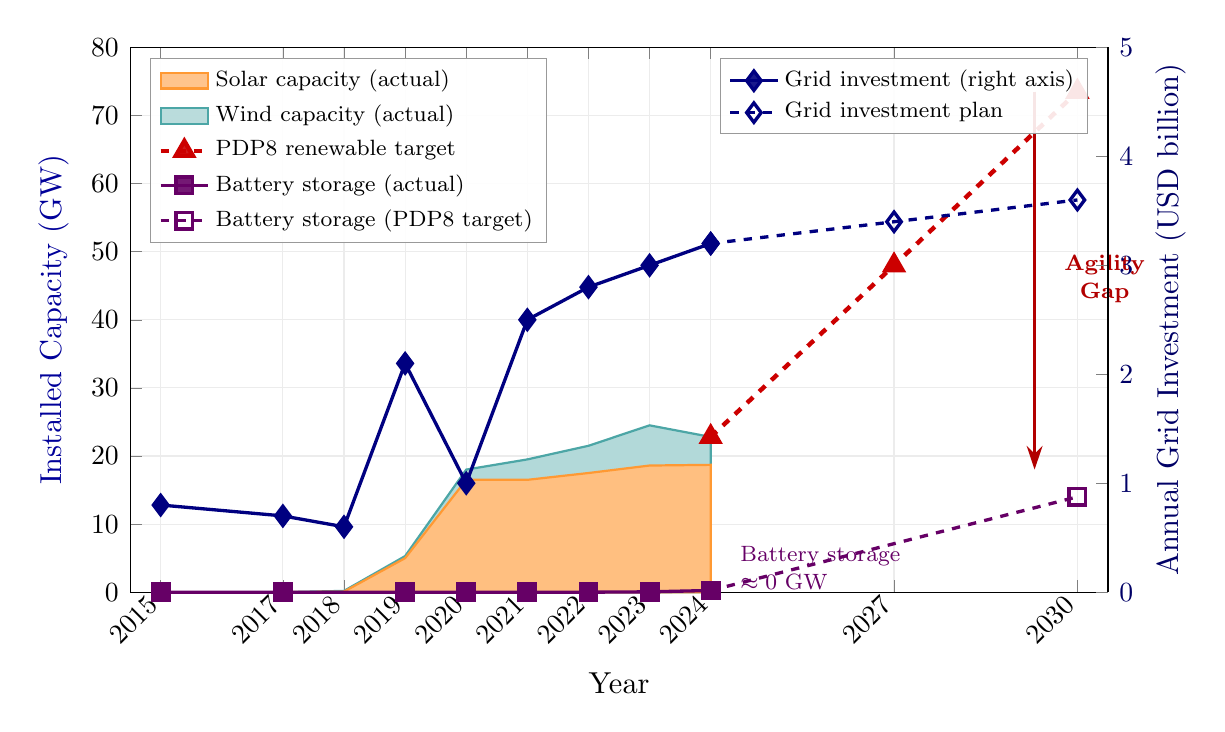
\begin{tikzpicture}
			\pgfplotsset{every x tick label/.append style={/pgf/number format/1000 sep={}}}
			\begin{axis}[
				name=mainaxis,
				width=14cm, height=8.5cm,
				xlabel={Year},
				ylabel={Installed Capacity (GW)},
				axis y line*=left,
				ylabel style={blue!60!black, font=\small},
				xmin=2014.5, xmax=2030.5,
				ymin=0, ymax=80,
				xtick={2015,2017,2018,2019,2020,2021,2022,2023,2024,2027,2030},
				xticklabel style={rotate=45, anchor=east, font=\footnotesize},
				ytick={0,10,20,30,40,50,60,70,80},
				xlabel style={font=\small},
				tick label style={font=\footnotesize},
				legend style={at={(0.02,0.98)}, anchor=north west, font=\scriptsize,
					draw=black!40, fill=white, fill opacity=0.9, text opacity=1,
					cells={anchor=west}, row sep=1pt},
				grid=major,
				grid style={gray!15},
				clip=false,
				]
				
				% --- Stacked area: Wind on top of Solar ---
				% Wind layer (total = solar + wind): draw this FIRST so solar overlays
				\addplot[fill=teal!30, draw=teal!70, thick, area legend, forget plot] coordinates {
					(2015, 0.004) (2017, 0) (2018, 0.19) (2019, 5.3) (2020, 18.0)
					(2021, 19.5) (2022, 21.5) (2023, 24.5) (2024, 22.8)
				} \closedcycle;
				
				% Solar layer (bottom of stack)
				\addplot[fill=orange!50, draw=orange!80, thick, area legend, forget plot] coordinates {
					(2015, 0.004) (2017, 0) (2018, 0.086) (2019, 5.0) (2020, 16.5)
					(2021, 16.5) (2022, 17.5) (2023, 18.6) (2024, 18.7)
				} \closedcycle;
				
				% Dummy entries for legend (correct order)
				\addlegendimage{area legend, fill=orange!50, draw=orange!80, thick}
				\addlegendentry{Solar capacity (actual)}
				\addlegendimage{area legend, fill=teal!30, draw=teal!70, thick}
				\addlegendentry{Wind capacity (actual)}
				
				% PDP8 renewable target path (dashed)
				\addplot[red!80!black, ultra thick, dashed, mark=triangle*, mark size=3.5pt,
				mark options={solid, fill=red!80!black}] coordinates {
					(2024, 22.8) (2027, 48.0) (2030, 73.5)
				};
				\addlegendentry{PDP8 renewable target}
				
				% Battery storage actual (violet, solid)
				\addplot[violet!80!black, very thick, mark=square*, mark size=3pt,
				mark options={solid, fill=violet!80!black}] coordinates {
					(2015, 0) (2017, 0) (2019, 0) (2020, 0) (2021, 0) (2022, 0)
					(2023, 0.05) (2024, 0.25)
				};
				\addlegendentry{Battery storage (actual)}
				
				% Battery storage PDP8 target (violet, dashed)
				\addplot[violet!80!black, very thick, dashed, mark=square, mark size=3pt,
				mark options={solid, draw=violet!80!black}] coordinates {
					(2024, 0.25) (2030, 14.0)
				};
				\addlegendentry{Battery storage (PDP8 target)}
				
				% Annotation arrow: agility gap at 2030
				\draw[-{Stealth[length=3mm, width=2mm]}, red!70!black, line width=1.2pt]
				(axis cs:2029.3, 73.5) -- (axis cs:2029.3, 18);
				\node[red!70!black, font=\scriptsize\bfseries, anchor=west] at (axis cs:2029.6, 46)
				{\shortstack{Agility\\Gap}};
				
				% Annotation: battery near zero
				\node[violet!80!black, font=\scriptsize, anchor=west] at (axis cs:2024.3, 3.5)
				{\shortstack[l]{Battery storage\\$\approx 0$~GW}};
				
			\end{axis}
			
			% Right y-axis: Grid investment (overlaid axis)
			\begin{axis}[
				width=14cm, height=8.5cm,
				axis y line*=right,
				axis x line=none,
				xmin=2014.5, xmax=2030.5,
				ymin=0, ymax=5,
				ylabel={Annual Grid Investment (USD billion)},
				ylabel style={blue!40!black, font=\small},
				ytick={0,1,2,3,4,5},
				yticklabel style={font=\footnotesize, blue!40!black},
				legend style={at={(0.98,0.98)}, anchor=north east, font=\scriptsize,
					draw=black!40, fill=white, fill opacity=0.9, text opacity=1,
					cells={anchor=west}},
				]
				
				% Grid investment actual
				\addplot[blue!50!black, very thick, mark=diamond*, mark size=3.5pt,
				mark options={solid, fill=blue!50!black}] coordinates {
					(2015, 0.8) (2017, 0.7) (2018, 0.6) (2019, 2.1) (2020, 1.0)
					(2021, 2.5) (2022, 2.8) (2023, 3.0) (2024, 3.2)
				};
				\addlegendentry{Grid investment (right axis)}
				
				% Grid investment PDP8 plan
				\addplot[blue!50!black, very thick, dashed, mark=diamond, mark size=3.5pt,
				mark options={solid, draw=blue!50!black}] coordinates {
					(2024, 3.2) (2027, 3.4) (2030, 3.6)
				};
				\addlegendentry{Grid investment plan}
				
			\end{axis}
		\end{tikzpicture}
		\caption[Descriptive Evidence for the Agility Gap]{Descriptive evidence for the agility gap. Left axis: installed renewable capacity (GW), decomposed into solar (orange) and wind (teal). Capacity surged from near-zero in 2017 to 22.8~GW by 2024; PDP8 targets 73.5~GW by 2030. Right axis: annual grid transmission investment (USD billion), which grew modestly from \$0.6--\$0.8B to \$3.2B. Battery storage (violet) remained near zero through 2024 despite a PDP8 target of 14~GW by 2030. Data: \citep{mof2023} (PDP8), \citep{evn2023}, \citep{iea2023}.}
		\label{fig:agility_gap_descriptive}
	\end{figure}
	
	\section{Literature Review}
	There has been a significant amount of environmental policy research utilizing DSGE models to analyze macroeconomic variables.\footnote{See \citep{annicchiarico2015}, \citep{dissou2016}, \citep{annicchiarico2017}, \citep{khan2019}, \citep{chan2020a}, \citep{chan2020b}, \citep{lintunen2021}, and \citep{xiao2022}.}A central debate in E-DSGE research concerns the optimal instrument for emission control under uncertainty. \citet{fischer2011} and \citet{bosetti2013} argue that carbon taxes generally outperform quantity-based instruments (like cap-and-trade) by reducing volatility in critical macroeconomic indicators and effectively lowering emissions. However, other scholars emphasize that these policies cannot be static; \citet{heutel2012} demonstrates that optimal environmental policy must adjust pro-cyclically with the business cycle to mitigate recessionary impacts. More recently, attention has shifted to how these policies interact with structural frictions. For instance, \citet{chan2023} reveals that the complementarity between energy and capital amplifies the transmission of shocks, 	suggesting that welfare-maximizing carbon taxes must be calibrated lower when endogenous capital utilization is taken into account.
	
	Existing environmental DSGE (E-DSGE) frameworks typically allow for imperfect substitution between energy and other inputs through CES aggregation, following \citet{heutel2012}. However, they overlook the non-linear costs of grid instability arising from renewable intermittency. Furthermore, most endogenous growth models in this domain, such as \citet{acemoglu2012environment}, focus on the inter-sectoral choice between ``clean'' and ``dirty'' production technologies, neglecting the intra-sectoral challenge of grid integration.
	
	There remains a critical gap in the literature regarding the interaction between renewable intermittency, investment frictions, and induced innovation. Specifically, current models fail to address how a developing economy manages the agility gap, the divergence between the rapid deployment of private renewable assets and the slow accumulation of public transmission infrastructure. Addressing this question requires a framework that explicitly endogenizes grid reliability and allows technological progress to respond to the shadow price of flexibility through a scarcity-induced innovation mechanism.
	
	Recently, \citet{airaudo2025green} advanced the Environmental DSGE literature by introducing a New Keynesian small open economy model that captures the macroeconomic costs of the green transition. Their analysis reveals that carbon taxes reduce brown energy use but cause short-term inflation and output losses, a phenomenon they term ``greenflation'', due to limited short-run substitutability between energy and traditional inputs. Crucially, they explicitly model public green investment as a fiscal instrument that can boost the productivity of the green sector. Their findings suggest that while carbon taxes alone are contractionary, mixed strategies that recycle carbon revenues into green public investment yield comparable environmental outcomes at lower welfare costs. 
	
	While \citet{airaudo2025green} focus on the short-run frictional costs of carbon taxation and fiscal policy coordination, this capstone complements their analysis by examining a distinct medium-run friction: the reliability penalty arising from renewable intermittency when flexibility infrastructure lags deployment. Whereas their greenflation emerges from incomplete factor substitutability under carbon pricing, the present model identifies an additional channel, endogenous grid instability, that operates even absent explicit carbon taxes, driven instead by the physical characteristics of VRE integration. This insight directly informs the policy discussion in Section \ref{sec:conclusion}.
	
	A distinct strand of literature rooted in endogenous growth theory offers a mechanism for long-run technological progress through innovation. The idea that factor scarcity directs innovation toward the scarce factor dates to \citet{hicks1932} and was formalized by \citet{kennedy1964} and \citet{drandakisphelps1966}. The modern Directed Technical Change (DTC) framework of \citet{acemoglu2002}, applied to energy by \citet{acemoglu2012environment}, models innovation as a resource allocation problem governed by two competing forces: the market size effect, which favors the larger sector, and the price effect, which favors the higher-priced sector. In the standard model the market size effect dominates, locking the economy into dirty technologies, but policy intervention can redirect innovation toward clean alternatives. Closest to the present paper, \citet{hassler2021} develop a DTC model in which natural resource scarcity endogenously redirects technological change away from energy-intensive inputs, demonstrating that physical scarcity, not just price signals, can serve as the directing force for innovation.
	
	This theoretical mechanism has found robust empirical support. \citet{popp2002} provided early evidence that higher energy prices significantly induce energy-efficient patenting activity. More recently, \citet{aghion2016} utilized microdata from the global automotive industry to show that firms tend to innovate in areas where they have prior expertise (path dependence), but that fuel price shocks successfully redirect R\&D toward electric and hybrid technologies. Similarly, \citet{calel2016} finds that firms regulated under the EU Emissions Trading System (ETS) increased low-carbon patenting by 10\% compared to a matched control group without crowding out other R\&D, suggesting that policy can effectively steer the direction of technical progress.
	
	However, a fundamental limitation in standard DTC models is the assumption regarding the elasticity of substitution. The AABH framework relies on the premise that clean and dirty inputs are high substitutes. Under this condition, innovation in clean energy allows it to seamlessly replace fossil fuels. Yet, structural analyses challenge this assumption in the presence of intermittency. As renewable penetration rises, the lack of dispatchability renders clean energy an imperfect substitute for baseload fossil generation \citep{hirth2013, joskow2011}. Consequently, models that treat clean capital as a homogeneous block overlook the necessity of complementary innovations. As argued by \citet{hart2019}, when inputs are complements rather than substitutes, technological progress must target not just generation, but the bottleneck technologies, specifically storage, that enable substitutability.
	
	An alternative mechanism for technological progress is learning-by-doing, where costs decline through accumulated production experience rather than explicit R\&D allocation. \citet{arrow1962} first formalized this idea, and it has been widely applied to renewable energy technologies. \citet{nemet2006} documents dramatic cost reductions in solar photovoltaics driven by cumulative deployment, while \citet{kittner2017} shows similar patterns for battery storage using a two-factor learning curve that integrates both deployment experience and innovation activity. \citet{way2022} extend this approach with stochastic Wright's Law forecasts across fifty technologies, projecting continued steep cost declines for batteries through 2050. Unlike DTC, learning-by-doing does not require modeling innovation sectors or resource constraints, making it particularly suitable for capturing technological progress in capital goods like batteries where costs decline through manufacturing scale and operational experience.
	
	To address these dynamics, recent contributions have attempted to internalize these physical constraints within general equilibrium frameworks. For instance, \citet{schreiner2020investing} develop a DSGE model for Germany that treats power grid infrastructure as a flexibility option required to bridge the mismatch between variable renewable supply and demand. Crucially, their simulations reveal that while grid investments increase reliability, the associated costs can lead to long-term decreases in GDP and employment unless accompanied by significant efficiency gains. This underscores that solving the intermittency problem is not merely a matter of capital accumulation (building more lines) but requires targeted technological progress in intertemporal substitution (storage).
	
	While the engineering literature has long established the necessity of storage for renewable integration, macroeconomic frameworks have lagged in formally modeling this investment channel. Techno-economic analyses, such as \citet{zakeri2015} and \citet{lund2015}, demonstrate that, as renewable penetration increases, the primary cost driver shifts from generation (LCOE) to flexibility (integration costs). They argue that, without storage, the social cost of intermittency rises nonlinearly due to the need for redundant fossil-fuel backup.
	
	Despite this, the standard E-DSGE literature largely omits storage as an endogenous decision variable. Major recent contributions, including \citet{batten2020} and \citet{annicchiarico2021}, focus predominantly on pricing instruments (carbon taxes) or quantity restrictions (caps), effectively assuming that energy markets clear instantaneously. When backup is modeled, as in \citet{schreiner2020investing}, it is often treated as a static infrastructure cost or fossil generation, which inherently reintroduces carbon emissions or capital rigidities that dampen the efficacy of green transition policies.
	
	This creates a significant modeling gap. By treating backup as fossil generation rather than intertemporal substitution, existing models fail to capture the capital-intensive nature of grid stability. As noted by \citet{kittner2017}, the declining costs of battery technologies imply that energy storage is transitioning from a niche ancillary service to a core infrastructure asset. Consequently, accurately capturing the greenflation trade-off requires a framework where agents can optimize investment not just in productive capital, but also in smoothing capital (BESS), a structural feature this capstone seeks to integrate.
	
	Beyond the storage modeling gap, international trade is a critical transmission channel for small open economies like Vietnam. Energy price shocks behave like terms-of-trade shocks, generating persistent effects on output and external balances \citep{obstfeld1995, corsetti2010}, while cross-border carbon pricing raises leakage and competitiveness risks \citep{bohringer2018, balke2022}. For Vietnam specifically, dependence on imported coal and LNG makes global fossil-fuel prices a direct source of production-cost volatility \citep{iea2023, gso2024}, and energy-intensive export sectors face growing exposure to policies like the EU Carbon Border Adjustment Mechanism \citep{ec2023}. Empirical work confirms that trade openness interacts strongly with renewable adoption and emissions in comparable emerging economies \citep{almulali2015, vo2020}, underscoring that international linkages are a defining structural feature of Vietnam's green transition rather than a peripheral consideration.
	
	Taken together, the literature leaves a critical gap at the intersection of renewable intermittency, endogenous grid reliability, and scarcity-induced innovation, precisely the nexus this capstone addresses. The three contributions of this study directly target these gaps. First, by jointly
	modeling an explicit energy sector with endogenous grid reliability, I address the failure of existing E-DSGE frameworks to capture the non-linear costs of grid instability arising from renewable intermittency. Second, by integrating scarcity-induced technological change with investment frictions, I respond to the neglect of the intra-sectoral grid-integration challenge in endogenous growth models and the omission of storage as an endogenous decision variable in standard
	macroeconomic frameworks. Third, by providing a second-best policy analysis conditional on
	the transmission of scarcity signals, I examine how a developing economy manages the agility gap
	(the divergence between rapid private renewable deployment and slow public infrastructure accumulation) that current models fail to address. The model developed in the next section fills
	these gaps by jointly endogenizing the reliability constraint, battery technological change, and
	the asymmetric investment dynamics that produce the agility gap.
	
	
	\section{The Model} \label{sec:methodology}
	
	\subsection{Model Overview}
	
	I develop a Small Open Economy Dynamic Stochastic General Equilibrium (DSGE) model calibrated to Vietnam. The model is designed to analyze the macroeconomic consequences of renewable-energy intermittency when the accumulation of grid flexibility lags behind the expansion of variable renewable generation, while capturing the external balance implications through international borrowing and lending. The framework extends standard Environmental DSGE (E-DSGE) models by introducing two departures from the canonical structure.
	
	First, grid reliability is endogenized as a technological constraint on effective capital services rather than treated implicitly through energy prices or exogenous productivity shocks. This reflects the physical reality that electricity systems with high renewable penetration are constrained by temporal mismatches between supply and demand. Second, I embed a scarcity-induced technological change mechanism that governs the rate of improvement in battery storage technologies. This allows the economy to respond endogenously to reliability scarcity through technological progress rather than relying solely on capital accumulation or policy intervention.
	
	The economy consists of a representative household and a representative firm operating in a small open economy with access to international bond markets. Households supply labor, accumulate productive capital, and trade bonds with the rest of the world at a debt-elastic interest rate. Firms produce final output using a CES aggregator of value-added (from capital and labor) and a fixed energy endowment. Grid reliability is determined endogenously by the stock of flexibility assets (batteries and grid infrastructure) relative to renewable volatility. Battery technology improves through scarcity-induced innovation driven by reliability gaps, while public grid investment follows a rule-based response to reliability shortfalls.
	
	A central modeling choice is the treatment of capital utilization. In contrast to standard RBC or New Keynesian models, capital utilization in this framework is not a choice variable and does not affect depreciation. Instead, it reflects the fraction of installed productive capital that is operational given the state of grid reliability. This interpretation aligns utilization with system-wide power availability rather than firm-level intensity of use.
	
	\subsection{Households} \label{sec:households}
	
	A representative household maximizes expected lifetime utility:
	\begin{equation}
		\mathbb{E}_0 \sum_{t=0}^{\infty} \beta^t
		\left[
		\log(C_t) - \varphi \frac{L_t^{1+\sigma_L}}{1+\sigma_L}
		\right]
		\label{eq:utility},
	\end{equation}
	
	subject to the budget constraint:
	\begin{equation}
		C_t + I_{p,t} + P_{bat,t} I_{bat,t} + B^*_t + \tau Y_t + T_t
		=
		w_t L_t + R_t K_{p,t-1} + \Pi_t + (1+r^*_{t-1}) B^*_{t-1}
		\label{eq:hh_budget},
	\end{equation}
	
	where $\tau$ is the fixed proportional tax rate, $T_t$ is a residual lump-sum tax (or transfer) that balances the government budget dynamically ($I_{grid,t} = \tau Y_t + T_t$), $w_t$ the real wage, $R_t$ the rental rate on $K_{p,t-1}$, $\Pi_t$ the rents from the exogenous energy endowment, and $B^*_t$ net foreign assets.\footnote{\label{fn:timing_convention}Capital installed at $t-1$ is productive in $t$; investment $I_{p,t}$ does not contribute until $t+1$.}

The household chooses $\{C_t, L_t, K_{p,t+1}, B^*_t\}$ to maximize utility subject to the budget constraint \eqref{eq:hh_budget} and the standard capital accumulation law \eqref{eq:productive_capital}; the mathematical derivation is in Appendix~\ref{app:deriv_euler}.
	
	
\paragraph{Euler equation.} With proportional taxation, the after-tax return to capital in period $t+1$ is $(1-\tau)\alpha Y_{t+1}/K_{p,t}$, where $\tau$ is the fixed tax rate. The intertemporal optimality condition becomes:\footnote{The mathematical derivation is in Appendix~\ref{app:deriv_euler}.}
	\begin{equation}
		\frac{1}{C_t} = \beta \mathbb{E}_t \left[ \frac{(1-\tau)\,\alpha Y_{t+1}/K_{p,t} + 1 - \delta_p}{C_{t+1}} \right]
		\label{eq:euler}.
	\end{equation}
	
	The tax wedge $\tau$ shifts the steady-state capital stock downward but does not amplify shock dynamics beyond the standard Euler mechanism.
	
	\paragraph{Labor supply.} With the proportional tax, the household equates the marginal disutility of labor to the after-tax marginal utility of income. Substituting the competitive wage $w_t = (1-\alpha)V_t/L_t$:\footnote{The mathematical derivation is in Appendix~\ref{app:deriv_labor}.}
	\begin{equation}
		(1-\tau)(1-\alpha) V_t = \varphi \, C_t \, L_t^{1+\sigma_L}
		\label{eq:labor_supply}.
	\end{equation}
	
	The parameter $\varphi$ is calibrated endogenously to match steady-state labor hours $L_{ss} = 0.33$.
	
	\subsection{The Production Sector}
	
	\subsubsection{Final Goods Production}
	
	Final output $Y_t$ is produced by a representative firm using a nested Constant Elasticity of Substitution (CES) technology that combines value-added and energy inputs. To reduce notational clutter in the CES expressions that follow, I adopt the convention of writing exponents in terms of the substitution parameter $s \equiv (\sigma - 1)/\sigma$ for a given elasticity $\sigma$. When $\sigma < 1$ (complements), $s < 0$; when $\sigma > 1$ (substitutes), $s > 0$; when $\sigma = 1$ (Cobb-Douglas), $s = 0$. Using $s_E \equiv (\sigma_E - 1)/\sigma_E$ for the output aggregator:
	
	\begin{equation}
		Y_t = \left[(1-\omega_E)V_t^{s_E} + \omega_E \bar{E}^{s_E}\right]^{1/s_E}
		\label{eq:final_output}.
	\end{equation}
	
	When $\sigma_E = 0.6 < 1$, energy and value-added are gross complements: disruptions to energy supply translate into disproportionately large output losses \citep{heutel2012}.

Value-added production combines labor and effective capital services:
	
	\begin{equation}
		V_t = Z\,(u_t K_{p,t-1})^\alpha L_t^{1-\alpha}
		\label{eq:value_added}.
	\end{equation}
	
	Effective capital $u_t K_{p,t-1}$ is the operational fraction of installed capacity ($u_t \in (0,1)$, capturing system-wide outages rather than a firm-level choice): a 3\% reliability shortfall is equivalent to a TFP loss of $\alpha \times 3\%\approx 1\%$.

Energy enters as a fixed endowment $\bar{E}$ (PDP8 targets); the intermittency shock propagates through the reliability function rather than energy supply directly.
	
	\subsection{Grid Reliability and Flexibility Assets}
	
	\subsubsection{Reliability Constraint}
	
	The reliability constraint is formalized as:
	
	\begin{equation}
		u_t = 1 - \exp\left(-\psi \frac{F_t}{\phi_{int} \cdot \text{Vol}_{ren,t}}\right)
		\label{eq:utilization}.
	\end{equation}
	
	Grid reliability is an increasing, concave function of the ratio of flexibility assets ($F_t$) to renewable volatility ($\text{Vol}_{ren,t}$). When the system has abundant flexibility relative to volatility, nearly all capital can operate ($u_t \approx 1$); when flexibility is scarce, outages proliferate and utilization collapses.
	
	This exponential form is standard in reliability engineering \citep{zakeri2015, lund2015}: $u_t \in (0,1)$ for all $F_t > 0$, reliability is bounded between grid collapse and perfection, and marginal returns to flexibility are strictly diminishing.
	
	Table~\ref{tab:reliability_numerical} in Appendix~\ref{app:reliability} illustrates this nonlinearity: a 10\% flexibility deficit reduces reliability by 1.26~pp, but a 50\% deficit causes a 14.32~pp collapse. The accelerating penalty motivates the Reliability Valley analysis in Section~\ref{sec:results}.
	
	The volatility term captures the absolute variability of renewable generation:
	\begin{equation}
		\overline{\text{Vol}}_{ren} = \theta_{ren} \cdot K_{ren} \cdot \sigma_{ren}
		\label{eq:renewable_volatility},
	\end{equation}
	
	where $\theta_{ren}$, $K_{ren}$, and $\sigma_{ren}$ are the penetration share, installed capacity, and CV of the intermittency shock. The shock $\varepsilon_{ren,t}$ enters multiplicatively as $\overline{\text{Vol}}_{ren}\cdot\exp(\varepsilon_{ren,t})$; in transition simulations $\overline{\text{Vol}}_{ren}$ rises with VRE expansion.
	
	\subsubsection{Public and Private Flexibility Assets}
	
	Total system flexibility $F_t$ combines private battery storage (time-shifting) and public grid (space-shifting) via a CES aggregator:

	\begin{equation}
		F_t =
		\left[
		\mu (A_{bat,t-1} K_{b,t-1})^{s_F}
		+
		(1-\mu) K_{g,t-1}^{s_F}
		\right]^{1/s_F},
		\qquad \rho < 1 \;\Leftrightarrow\; s_F < 0
		\label{eq:flexibility_bundle}.
	\end{equation}
	
	The negative exponent $s_F<0$ ($\rho=0.4<1$) enforces imperfect complementarity; all inputs are predetermined from period $t-1$. See Proposition~\ref{prop:superadditivity} (Appendix~\ref{app:proof_superadditivity}).
	
	\subsubsection{Laws of Motion}
	
	Public grid capital evolves according to a standard accumulation equation:
	
	\begin{equation}
		K_{g,t+1} = (1-\delta_g)K_{g,t} + I_{grid,t}
		\label{eq:grid_capital}.
	\end{equation}
	
	Grid investment is undertaken by the government and is subject to institutional inertia, reflecting planning delays and construction lags. As a result, public flexibility adjusts slowly to changes in renewable penetration.
	
	Private battery capital evolves as:
	
	\begin{equation}
		K_{b,t+1} = (1-\delta_b)K_{b,t} + I_{bat,t}
		\label{eq:battery_capital}.
	\end{equation}
	
	Battery capital follows a standard linear accumulation law without adjustment costs, as the modular and scalable nature of battery storage allows rapid deployment without the installation frictions typically associated with heavy infrastructure.
	
	\paragraph{Battery Investment Decision.}
	The investment rule below proxies the gradient of the structural shadow price while preserving local saddle-path stability; the mathematical derivation is in Appendix~\ref{app:deriv_euler}.

	Table~\ref{tab:mpk_decomp} evaluates the shadow rental rate at steady state, yielding $R_{b,ss} = 10.93\%$ quarterly. The flexibility bottleneck ($\partial F / \partial(A_{bat} K_b) = 2.04$) is the dominant force, reflecting battery scarcity in the CES aggregator, while the reliability gradient is moderate because the system operates near $u_{ss} = 0.97$.
	
	\begin{table}[H]
		\centering
		\caption[Marginal Product Decomposition of Battery Rental Rate]{\textbf{Marginal Product Decomposition of Battery Rental Rate ($R_{b,ss}$)}}
		\label{tab:mpk_decomp}
		\renewcommand{\arraystretch}{1.3}
		\small
		\begin{tabular}{l l c l}
			\toprule
			\textbf{Component} & \textbf{Expression} & \textbf{Value} & \textbf{Interpretation} \\
			\midrule
			CES output share & $\partial Y / \partial V$ & 0.725 & Value-added dominates output \\
			Utilization effect & $\partial V / \partial u = \alpha V/u$ & 0.370 & Capital utilization channel \\
			Reliability gradient & $\partial u / \partial F$ & 0.200 & Moderate (near flat of exp.\ curve) \\
			Flexibility bottleneck & $\partial F / \partial (A_{bat} K_b)$ & 2.040 & Scarce factor in CES \\
			\midrule
			\textbf{Shadow rental rate} & $R_{b,ss}$ & \textbf{0.109} & \textbf{10.93\% quarterly} \\
			\bottomrule
		\end{tabular}
		\vspace{0.2cm}
		\parbox{\textwidth}{\footnotesize \textit{Note:} Evaluated at the deterministic steady state. $R_{b,ss} = (\partial Y/\partial V) \times (\partial V/\partial u) \times (\partial u/\partial F) \times (\partial F/\partial(A_{bat} K_b)) \times A_{bat} = 0.725 \times 0.370 \times 0.200 \times 2.040 \times 1.0 = 0.109$. The large flexibility bottleneck term reflects batteries' position as the scarce factor ($\mu = 0.16$) in the CES aggregator. When $u_t$ falls below target, the reliability gradient steepens (since $\partial u/\partial F \propto (1-u_t)$), amplifying $R_b$ and triggering the investment response.}
	\end{table}
	
	Rising reliability gap $(1-u_t)$ steepens the gradient and raises $R_{b,t}$, motivating:

	\begin{equation}
		\frac{I_{bat,t}}{\bar{I}_{bat}} = \left(\frac{u^*}{u_t}\right)^{\phi_{grid}} \cdot \frac{1}{P_{bat,t}}
		\label{eq:battery_investment}.
	\end{equation}
	
	Higher $\phi_{grid}$ implies more aggressive deployment when the grid is stressed; the price term $1/P_{bat,t}$ reflects Vietnam's price-taking position in global markets.
	
	\subsection{Scarcity-Induced Technological Change in Battery Storage}
	
	Battery technology evolves through scarcity-induced learning: when reliability falls below target, the return to improving storage rises and innovation accelerates \citep{hicks1932, acemoglu2002}. The law of motion is:
	\begin{equation}
		A_{bat,t} = A_{bat,t-1} \times \left(1 + \eta_{bat} \cdot \chi \cdot \frac{u^* - u_t}{u^*}\right)
		\label{eq:learning_by_doing},
	\end{equation}
	
where $\eta_{bat}$ is the innovation elasticity, $\chi\in(0,1]$ captures regulatory signal attenuation, and $u^*$ is the reliability target. Innovation is zero at $u_t=u^*$, accelerates when reliability falls below target, and enters $F_{t+1}$ with a one-period delay eliminating within-period simultaneity.

\subsection{Government} \label{sec:government}
	
	The government does not solve a Ramsey optimization problem. Instead, it follows an institutional reliability-targeting rule motivated by Vietnam's Power Development Plan 8 (PDP8). Public grid investment responds mechanically to deviations of reliability from a target level:
	
	\begin{equation}
		\frac{I_{grid,t}}{\bar{I}_{grid}} =
		\left(\frac{u^*}{u_t}\right)^{\phi_{grid}}
		\exp(\varepsilon_{I,t})
		\label{eq:grid_investment_rule}.
	\end{equation}
	
	The government spends more on grid infrastructure when reliability falls below target, and less when the grid is performing well. This rule is structurally identical to the battery investment rule \eqref{eq:battery_investment} except that it lacks a price term (grid investment uses domestically produced goods) and includes an implementation shock $\varepsilon_{I,t}$ reflecting bureaucratic delays, procurement bottlenecks, and construction lags.
	
	This rule captures the reactive nature of infrastructure policy, where investment accelerates following reliability crises rather than anticipating them. The parameter $\phi_{grid}$ governs the aggressiveness of the fiscal response.
	
	The government finances grid investment through a fixed proportional tax $\tau_{ss}=I_{grid,ss}/Y_{ss}=1.43\%$ ($\tau_{ss}=\delta_g K_{g,ss}/Y_{ss}=0.0143$), ensuring tax revenue covers replacement grid investment.

	\subsection{Battery Price Dynamics}
	
	Battery investment goods are priced at world price $P_{bat,t}$, which enters the resource constraint and the battery investment rule. The world price of batteries evolves according to a persistent AR(1) process:
	\begin{equation}
		\log P_{bat,t} = \rho_{bat} \log P_{bat,t-1} + \varepsilon_{bat,t}
		\label{eq:battery_price_shock},
	\end{equation}
	
	where $\varepsilon_{bat,t} \sim N(0, \sigma^2_{bat})$ captures global shocks to battery costs (e.g., lithium price volatility, supply chain disruptions). This channel allows the model to examine how external cost shocks to the green transition propagate through the domestic economy. In steady state, $P_{bat,ss} = 1$ (normalized).
	
	\subsection{External Sector}
	
	The model follows the debt-elastic interest rate approach of \citet{schmittgrohe2003}, giving the household access to international bond markets at a country-specific rate.

	\subsubsection{Bond Euler Equation}

	The household's optimality condition for international bond holdings yields:
	\begin{equation}
		\frac{1}{C_t} = \beta \, \mathbb{E}_t \left[ \frac{1 + r^*_t}{C_{t+1}} \right]
		\label{eq:bond_euler}.
	\end{equation}

	Combining with \eqref{eq:euler} delivers the no-arbitrage condition $(1-\tau)\alpha Y_{t+1}/K_{p,t} + 1 - \delta_p = 1 + r^*_t$, confirming that the domestic after-tax return equals the external borrowing rate in equilibrium.
	
	\subsubsection{Debt-Elastic Interest Rate Premium}

	The country-specific interest rate rises with external debt, following \citet{schmittgrohe2003}:
	\begin{equation}
		r^*_t = \bar{r} + \phi_b \left( \exp(\bar{B}^* - B^*_t) - 1 \right)
		\label{eq:interest_premium}.
	\end{equation}

	With $\bar{r} = 1/\beta - 1$ and $\bar{B}^* = 0$, this premium stabilizes the net foreign asset process and resolves the unit-root problem standard in small open economy models.
	
	\subsection{Resource Constraint and Market Clearing}
	
	Output equals domestic absorption plus net capital outflows:
	\begin{equation}
		Y_t = C_t + I_{p,t} + P_{bat,t} I_{bat,t} + I_{grid,t} + \underbrace{(B^*_t - (1+r^*_{t-1})B^*_{t-1})}_{\text{net capital outflow}}
		\label{eq:goods_market_clearing}.
	\end{equation}
	
	\noindent Investment in productive capital $I_{p,t}$ evolves as:
	\begin{equation}
		K_{p,t+1} = (1-\delta_p) K_{p,t} + I_{p,t}
		\label{eq:productive_capital}.
	\end{equation}
	
	\subsection{Equilibrium Definition} \label{sec:equilibrium}

	A competitive equilibrium for this economy is defined as sequences of 16 endogenous variables
	$$\{Y_t, C_t, L_t, K_{p,t}, K_{b,t}, K_{g,t}, I_{p,t}, I_{bat,t}, I_{grid,t}, u_t, F_t, A_{bat,t}, V_t, P_{bat,t}, B^*_t, r^*_t\}_{t=0}^{\infty}$$

	satisfying 16 independent equations (given exogenous shocks $\varepsilon_{ren,t}$, $\varepsilon_{bat,t}$, $\varepsilon_{I,t}$ and calibrated parameters including $\overline{\text{Vol}}_{ren}$):

	\begin{enumerate}
		\item Capital Euler equation: \eqref{eq:euler}
		\item Bond Euler equation: \eqref{eq:bond_euler}
		\item Labor market clearing: \eqref{eq:labor_supply}
		\item CES final output: \eqref{eq:final_output}
		\item Value-added production: \eqref{eq:value_added}
		\item Reliability function: \eqref{eq:utilization}
		\item CES flexibility aggregator: \eqref{eq:flexibility_bundle}
		\item Battery investment rule: \eqref{eq:battery_investment}
		\item Battery capital accumulation: \eqref{eq:battery_capital}
		\item Scarcity-induced technological change: \eqref{eq:learning_by_doing}
		\item Grid investment rule: \eqref{eq:grid_investment_rule}
		\item Grid capital accumulation: \eqref{eq:grid_capital}
		\item Productive capital accumulation: \eqref{eq:productive_capital}
		\item Current account / budget constraint: \eqref{eq:goods_market_clearing}
		\item Debt-elastic interest rate premium: \eqref{eq:interest_premium}
		\item Battery price process: \eqref{eq:battery_price_shock}
	\end{enumerate}

	\noindent The no-arbitrage condition $(1-\tau)\alpha Y_{t+1}/K_{p,t}+1-\delta_p=1+r^*_t$ and the domestic absorption identity \eqref{eq:goods_market_clearing} are derived from the equations above and do not constitute additional independent conditions. The renewable volatility $\overline{\text{Vol}}_{ren}$ (equation~\ref{eq:renewable_volatility}) is a calibrated parameter, not an endogenous variable. The system is exactly identified: 16 equations in 16 unknowns.

	\subsection{Steady State Characterization}
	The deterministic steady state is computed by setting all shocks to zero and solving the 16-equation system analytically. Key values are: $u_{ss} = 0.97$, $Y_{ss} = 1.0$ (normalised), $K_{p,ss} = 9.83$, $L_{ss} = 0.33$, $C_{ss}/Y_{ss} = 0.734$, and $I_{grid,ss}/Y_{ss} = 0.014$. Battery capital $K_{b,ss}$ and grid capital $K_{g,ss}$ are calibrated to match the flexibility bundle target; the full steady-state derivation is in Appendix~\ref{app:steadystate}.

	\section{Model Mechanisms} \label{sec:mechanics}
	
	This section derives the log-linearized equilibrium system, characterizes the steady state, and describes the transmission channels through which intermittency shocks propagate. The model is solved using first-order perturbation methods following the Dynare toolkit approach \citep{Adjemianetal2024}, implemented in Dynare 6 \citep{Adjemianetal2024}. The solution methodology follows \citet{uhlig1999} for analyzing nonlinear dynamic stochastic models through log-linearization around the deterministic steady state.
	
	\subsection{Mechanism Summary}
	
	The model generates five propagation channels. The first three correspond to its core novelties, endogenous reliability, scarcity-induced innovation, and asymmetric investment dynamics, while Channels 4 and 5 are additional structural features that shape the steady state and external exposure.
	
	\paragraph{Channel 1: Intermittency to Reliability to Output.}
	Renewable intermittency shocks $\varepsilon_{ren,t}$ reduce grid reliability $u_t$ by increasing the mismatch between supply and demand (through $\text{Vol}_{ren,t}$). Lower reliability directly reduces effective capital utilization, acting as a negative productivity shock that depresses output $Y_t$, raises the effective cost of capital, and lowers wages.
	
	\paragraph{Channel 2: Reliability Gap to Investment.}
	Reduced reliability widens the gap $u^*/u_t$, raising the return to battery storage and stimulating battery investment $I_{bat,t}$ through the investment rule \eqref{eq:battery_investment}. Grid investment responds through the government's fiscal rule \eqref{eq:grid_investment_rule}. The differential speed of response, private battery versus public grid, constitutes the agility gap.
	
	\paragraph{Channel 3: Reliability Gap to Scarcity-Induced Innovation to Productivity Gain.}
	The reliability gap also accelerates scarcity-induced technological change in battery storage (equation \eqref{eq:learning_by_doing}), increasing the effective productivity of storage services. This creates a virtuous cycle where scarcity induces both more investment and faster technological progress. However, when regulatory distortions dampen scarcity signals ($\chi < 1$), this innovation channel is attenuated, prolonging reliability shortfalls and amplifying macroeconomic volatility.
	
	\paragraph{Channel 4: The Fiscal Wedge Channel.}
	The fixed tax $\tau$ imposes a permanent wedge, reducing structural resilience without dynamic amplification.

	Together, these mechanisms generate endogenous transition dynamics in which reliability scarcity, innovation, fiscal distortions, and macroeconomic performance are jointly determined.
	
	\subsection{Transmission Channels}
	
	Figure \ref{fig:mechanism} summarizes the model's transmission channels. The three exogenous shocks propagate through distinct but interconnected pathways.
	
	\begin{figure}[H]
		\centering
		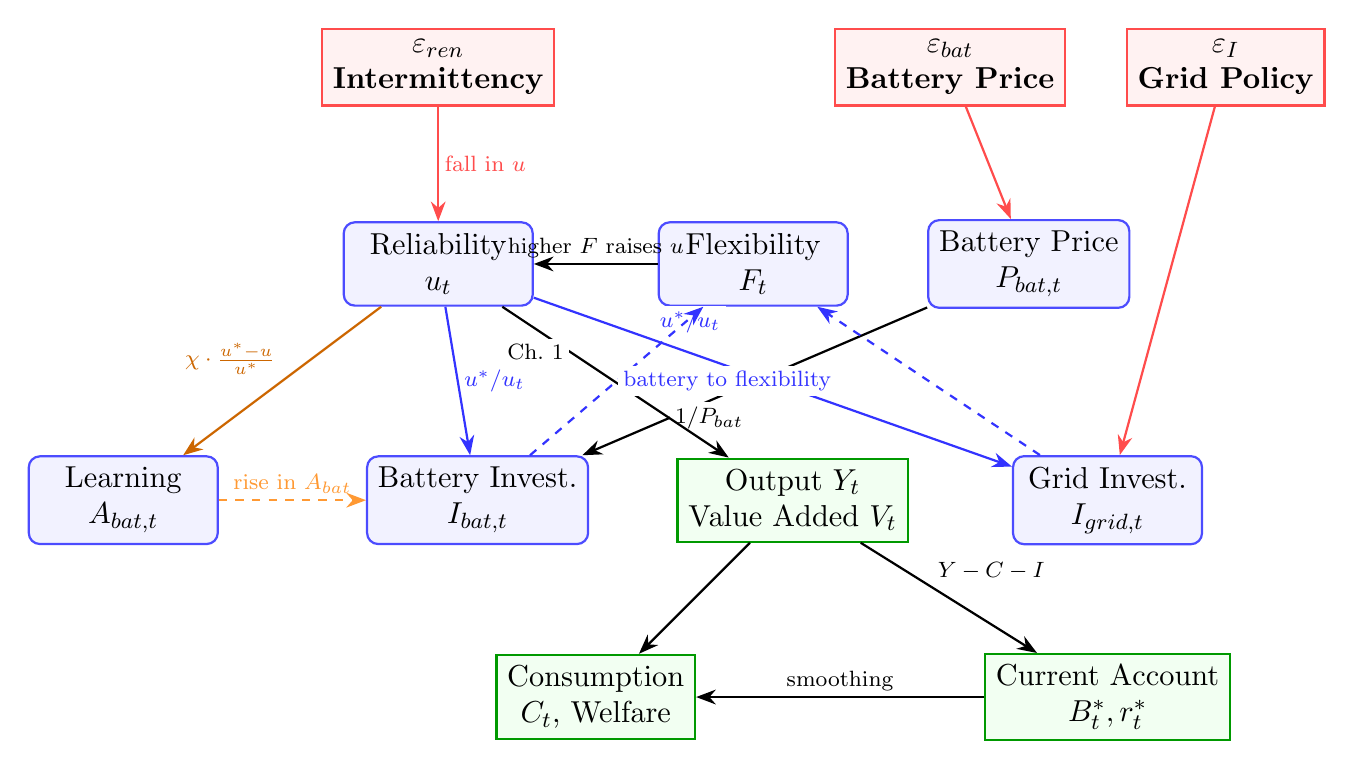
\begin{tikzpicture}[
			>={Stealth[length=2.5mm]},
			shock/.style={rectangle, draw=red!70, fill=red!5, thick, minimum width=2.4cm, minimum height=0.8cm, font=\small\bfseries, align=center},
			state/.style={rectangle, draw=blue!70, fill=blue!5, thick, rounded corners, minimum width=2.4cm, minimum height=0.8cm, font=\small, align=center},
			outcome/.style={rectangle, draw=green!60!black, fill=green!5, thick, minimum width=2.4cm, minimum height=0.8cm, font=\small, align=center},
			label_text/.style={font=\scriptsize, inner sep=2pt, fill=white}
			]
			
			% Shocks (top row)
			\node[shock] (eps_ren) at (0, 2.5) {$\varepsilon_{ren}$\\Intermittency};
			\node[shock] (eps_bat) at (6.5, 2.5) {$\varepsilon_{bat}$\\Battery Price};
			\node[shock] (eps_I) at (10, 2.5) {$\varepsilon_I$\\Grid Policy};
			
			% Middle layer
			\node[state] (rel) at (0, 0) {Reliability\\$u_t$};
			\node[state] (flex) at (4, 0) {Flexibility\\$F_t$};
			\node[state] (Pbat) at (7.5, 0) {Battery Price\\$P_{bat,t}$};
			
			% Investment responses & Output layer
			\node[state] (learn) at (-4, -3) {Learning\\$A_{bat,t}$};
			\node[state] (Ibat) at (0.5, -3) {Battery Invest.\\$I_{bat,t}$};
			\node[outcome] (output) at (4.5, -3) {Output $Y_t$\\Value Added $V_t$};
			\node[state] (Igrid) at (8.5, -3) {Grid Invest.\\$I_{grid,t}$};
			
			% Bottom layer (External sector & Consumption)
			\node[outcome] (cons) at (2, -5.5) {Consumption\\$C_t$, Welfare};
			\node[outcome] (ext) at (8.5, -5.5) {Current Account\\$B^*_t, r^*_t$};
			
			% Arrows from shocks
			\draw[->, red!70, thick] (eps_ren) -- node[right, label_text, text=red!70, fill=none] {fall in $u$} (rel);
			\draw[->, red!70, thick] (eps_bat) -- (Pbat);
			\draw[->, red!70, thick] (eps_I) -- (Igrid);
			
			% Flexibility to reliability
			\draw[->, thick] (flex) -- node[above, label_text, fill=none] {higher $F$ raises $u$} (rel);
			
			% Reliability to learning (Channel 3)
			\draw[->, orange!80!black, thick] (rel) -- node[above left, label_text, text=orange!80!black, fill=none] {$\chi \cdot \frac{u^*-u}{u^*}$} (learn);
			\draw[->, dashed, orange!80, thick] (learn) -- node[above, label_text, text=orange!80, fill=none] {rise in $A_{bat}$} (Ibat);
			
			% Reliability gap to investment (Channel 2)
			\draw[->, blue!80, thick] (rel) -- node[right, label_text, text=blue!80, fill=none] {$u^*/u_t$} (Ibat);
			\draw[->, blue!80, thick] (rel) -- node[pos=0.25, above right, label_text, text=blue!80] {$u^*/u_t$} (Igrid);
			
			% Price to battery investment
			\draw[->, thick] (Pbat) -- node[pos=0.75, right, label_text] {$1/P_{bat}$} (Ibat);
			
			% Reliability to Output (Channel 1)
			\draw[->, thick] (rel) -- node[pos=0.3, left, label_text] {Ch.\ 1} (output);
			
			% Investment to flexibility (feedback)
			\draw[->, dashed, blue!80, thick] (Ibat) -- node[pos=0.5, right, label_text, text=blue!80] {battery to flexibility} (flex);
			\draw[->, dashed, blue!80, thick] (Igrid) -- (flex);
			
			% Output to consumption and external
			\draw[->, thick] (output) -- (cons);
			\draw[->, thick] (output) -- node[pos=0.4, above right, label_text] {$Y - C - I$} (ext);
			
			% External to consumption (borrowing)
			\draw[->, thick] (ext) -- node[above, label_text, fill=none] {smoothing} (cons);
			
		\end{tikzpicture}
		\caption[Model Transmission Mechanism]{\textbf{Model Transmission Mechanism}}
		\label{fig:mechanism}
		\parbox{\linewidth}{\footnotesize \textbf{Note:} Solid arrows indicate contemporaneous effects; dashed arrows indicate dynamic feedback through capital accumulation. Channel 1 (reliability penalty): intermittency reduces $u_t$, which lowers $V_t$ and $Y_t$. Channel 2 (agility gap): the reliability gap triggers asymmetric investment responses ($I_{bat}$ agile, $I_{grid}$ sluggish). Channel 3 (directed learning): the reliability gap induces $A_{bat}$ improvement, conditional on signal transmission $\chi$. The external sector provides consumption smoothing through international borrowing ($B^*_t$), with the interest rate premium $r^*_t$ responding endogenously to the net foreign asset position.}
	\end{figure}
	
	

	\subsection{Linearization}

Variables are expressed as log-deviations from steady state, denoted by hats: $\hat{x}_t \equiv \ln X_t - \ln X_{ss}$. The full system of 16 linearized equations is provided in Appendix~\ref{app:log_lin}. This section focuses purely on the novel transmission mechanisms that differentiate this framework from a standard real business cycle model.

\subsubsection{The Reliability Wedge and Output}

Since energy enters as a fixed endowment $\bar{E}$ (i.e., $\hat{E}_t = 0$), the log-linearized CES production function simplifies to:
	\begin{equation}
		\hat{Y}_t = (1-\omega_E) s_V^{\frac{\sigma_E - 1}{\sigma_E}} \hat{V}_t
		\label{eq:output_lin}.
	\end{equation}
	
	Output fluctuations are proportional to value-added fluctuations, with the proportionality constant determined by the energy share and the CES curvature. Because energy is fixed, all business-cycle variation in output comes through the value-added channel, and hence through the reliability mechanism that drives $\hat{V}_t$.
	
	Here $s_V \equiv V_{ss}^{(\sigma_E-1)/\sigma_E} / [V_{ss}^{(\sigma_E-1)/\sigma_E} + (\omega_E/(1-\omega_E)) \bar{E}^{(\sigma_E-1)/\sigma_E}]$ denotes the steady-state value-added share in the CES aggregate. The value-added component linearizes as:
	\begin{equation}
		\hat{V}_t = \alpha(\hat{u}_t + \hat{K}_{p,t-1}) + (1-\alpha)\hat{L}_t
		\label{eq:va_lin}.
	\end{equation}
	
	Reliability $\hat{u}_t$ enters value-added with elasticity $\alpha$ (a 1\% reliability drop reduces output by $\approx 0.35\%$). Linearizing the exponential reliability function around steady state yields the reliability wedge equation, with reliability elasticity $\xi \equiv \frac{1-u_{ss}}{u_{ss}} \cdot \psi \frac{F_{ss}}{\phi_{int} \cdot \text{Vol}_{ren,ss}}$:
	\begin{equation}
		\hat{u}_t = -\xi \cdot \hat{\varepsilon}_{ren,t}
		\label{eq:reliability_lin}.
	\end{equation}
	
	Under the baseline ($\xi \approx 0.26$), a 5\% adverse intermittency shock reduces utilization by $\approx$1.3~pp if flexibility does not adjust, the Agility Gap mechanism.	

	\noindent Full derivation in Appendix~\ref{app:log_lin}.

\subsubsection{Scarcity-Induced Technological Change}
The scarcity-induced innovation equation linearizes around steady state. Since $u_{ss} = u^*$, the reliability gap $(u^* - u_t)/u^*$ linearizes to $-\hat{u}_t$ (in log-deviations). Thus:
	\begin{equation}
		\underbrace{\hat{A}_{bat,t} - \hat{A}_{bat,t-1}}_{\text{technology growth}} = -\eta_{bat} \cdot \chi \cdot \hat{u}_t
		\label{eq:abat_lin}.
	\end{equation}
	
	Battery technology improves proportionally to the reliability shortfall, modulated by $\eta_{bat}=0.10$ and regulatory transmission $\chi$; suppressed signals or a healthy grid cause technology to stagnate. Full system in Appendix~\ref{app:log_lin}.	

	\paragraph{Interaction: The Reliability Valley.}
	The interaction of Channels 1--4 generates the Reliability Valley identified in the abstract. During a transition to high renewable penetration, the deterministic path of increasing intermittency outpaces both the sluggish accumulation of public grid capital (Channel 3) and the gradual improvement in storage technology (Channel 2). The resulting reliability shortfall persists for several years, during which households bear welfare losses through reduced consumption and increased energy price volatility. The depth and duration of the valley depend on the relative speed of private innovation versus public infrastructure accumulation, the Agility Gap.
	
	
	\section{Calibration} \label{sec:calibration}
	
	The model is calibrated at a quarterly frequency to capture the structural characteristics of the Vietnamese economy and the specific investment targets outlined in the Eighth Power Development Plan (PDP8). The calibration strategy proceeds in three stages: (i) standard structural parameters are set to match long-run moments of the Vietnamese economy; (ii) the novel reliability and intermittency parameters are micro-founded using engineering data from the General Statistics Office of Vietnam \citep{gso2024} and the International Energy Agency \citep{iea2023}; and (iii) innovation parameters are drawn from the empirical induced innovation literature. Table~\ref{tab:calibration} summarizes the baseline calibration.
	
	\subsection{Preferences and Production}
	I set the discount factor $\beta = 0.99$, implying an annualized real interest rate of 4\%, consistent with the average return on government bonds in emerging Asian economies. The capital share in the value-added function is set to $\alpha = 0.35$, matching the standard labor income share of 0.65 observed in Vietnam \citep{gso2024}. The depreciation rate of productive capital is set to $\delta_p = 0.025$ (10\% annually). The elasticity of labor supply is set to $\sigma_L = 1.0$, a standard value in the New Keynesian literature for developing economies.
	
	The elasticity of substitution between energy and value-added is set to $\sigma_E = 0.6$, following \citet{heutel2012} and consistent with empirical estimates for emerging economies where energy-capital complementarity is strong.
	
	\subsection{The Energy Transition Block}
	
	A core contribution of this capstone is the rigorous calibration of the reliability constraint, which is micro-founded on the physical properties of the Vietnamese grid rather than arbitrary assumptions.
	
	\subsubsection{Renewable Intermittency}
	
	Intermittency is calibrated to Vietnamese solar and wind data \citep{iea2023, gso2024}: persistence $\rho_{ren} = 0.85$ (monsoon-driven seasonal autocorrelation), volatility $\sigma_{ren} = 0.12$ (national fleet CV of monthly output), and bound $\varepsilon_{max} = 3\sigma_{ren}$ ensuring non-negativity with 99\% probability.

	\subsubsection{Flexibility Production Function}

	\paragraph{Flexibility Weight ($\mu = 0.16$).}
	Calibrated from PDP8 investment flows: the near-term battery share is $0.24/(0.24+1.49)\approx 0.14$, rising to $0.64$ in 2027--2030; the baseline adopts a conservative near-terminal value, robust to $\mu\in[0.12,0.20]$.

	\paragraph{Elasticity of Substitution ($\sigma_f = 0.4$).}
	Battery and grid are gross complements ($\sigma_f<1$): transmission moves power across space, storage across time, and neither alone delivers system reliability \citep{hart2019,hirth2013}.

	\paragraph{Reliability Function Parameters.}
	The exponential utilization function \eqref{eq:utilization} contains two key parameters: $\psi$ and $\phi_{int}$. The parameter $\psi=2.0$ is identified from the slope moment $\Delta u/(\Delta\ln F\cdot(1-u_{ss}))\approx 1.85$ (reliability rose 1.5~pp following a 20\% transmission expansion, 2016--2020 \citep{evn2023}); $\phi_{int}\approx 55.6$ is then pinned by the level condition $u_{ss}=0.97$. Both are robust for $\psi\in[1.5,3.0]$.
	
	
	\subsection{Technology Adoption Elasticity and Innovation}
	
		The technology adoption elasticity is set to $\eta_{bat} = 0.10$ (quarterly), within the 0.05--0.35 induced-innovation elasticity range estimated by \citet{popp2002} and consistent with the 18--22\% battery experience curve of \citet{kittner2017}. A sustained 10\% reliability gap in the model yields approximately 1\% quarterly battery efficiency improvement, matching the secular pace of cost reduction documented in \citet{way2022}.
	
	The baseline sets $\chi=1.0$ (full signal transmission); the regulated counterfactual uses $\chi=0.3$, calibrated to Vietnam's documented retail tariff pass-through of 25--35\% \citep{ieefa2022}.
	
	\subsection{Battery Price Shock Calibration}
	
	The world battery price shock follows $\rho_{bat} = 0.90$ and $\sigma_{bat} = 0.08$ (quarterly). The half-life of $\approx 6.6$ quarters (1.6 years) matches the 2--3 year lithium supply-demand adjustment cycle driven by mine development timelines \citep{bloombergnef2023}, and is consistent with BloombergNEF annual AR(1) estimates of 0.88--0.93 for quarterly-averaged battery pack prices.
	
	\subsection{Government and Fiscal Policy}
	The grid investment rule parameter $\phi_{grid} = 1.5$ is the semi-elasticity of public grid investment to reliability shortfalls, calibrated to Vietnam's fiscal response to the June 2023 power shortages \citep{evn2023,worldbank2022}. The fixed proportional tax rate $\tau_{ss} = 1.43\%$ finances steady-state grid maintenance ($I_{grid,ss}/Y_{ss} = \delta_g K_{g,ss}$).
	
	The grid investment implementation shock has AR(1) persistence $\rho_I = 0.70$ (quarterly, half-life $\approx$1.9 quarters) and standard deviation $\sigma_I = 0.05$.\footnote{$\varepsilon_{I,t}$ is a quarterly budget-execution shock, a temporary disruption to the disbursement rate of planned investment, not a shock to total project timelines. The 2--3 year completion delays in \citet{worldbank2022} are embedded in capital accumulation dynamics; the AR(1) shock captures quarterly disturbances (budget sequestration, contractor delays, procurement bottlenecks) that Ministry of Finance execution reports show resolve within one to two fiscal quarters \citep{mof2023}. The volatility $\sigma_I = 0.05$ (20\% annualized) matches the CV of annual public energy investment disbursements \citep{worldbank2022}.} 	Implementation shocks account for 82\% of grid investment variance (Appendix~\ref{app:fevd}), consistent with the view that public energy investment in Vietnam is primarily constrained by execution capacity rather than the reliability signal itself.
	
	\subsection{External Sector} \label{subsec:external_sector}

	The world interest rate is set to $\bar{r} = 1/\beta - 1 = 0.0101$ (quarterly), ensuring consistency with the household's Euler equation in steady state. The discount factor $\beta = 0.99$ is disciplined by Vietnam's historical real interest rate series \citep{worldbank2024}. Over the post-WTO modern era (2000--2023, 23 annual observations), the mean real rate on long-term government bonds was $3.14\%$ annually, implying $\beta = (1 + 0.0314)^{-1/4} \approx 0.9691 \approx 0.97$. The value $\beta = 0.99$ is slightly higher, corresponding to approximately $4\%$ annualized real returns; this conservative choice reflects Vietnam's current government borrowing costs and serves as a defensible anchor for fiscal policy analysis. Sensitivity to $\beta \in [0.95, 0.99]$ is documented in the robustness appendix.
	
	The debt-elastic premium $\phi_b = 0.039$ is estimated from Vietnam's real interest rate and external debt/GNI \citep{worldbank2024} by no-intercept OLS ($R^2 = 0.16$); $\phi_b = 0.039$ yields the credible $-3.5\%$ investment response vs.\ $-21.8\%$ at the SGU standard.

	\begin{table}[H]
		\centering
		\caption[Structural Parameter Calibration (Vietnam Scenario)]{\textbf{Structural Parameter Calibration (Vietnam Scenario)}}
		\label{tab:calibration}
		\renewcommand{\arraystretch}{1.3}
		\small
		\begin{tabular}{l c l p{6.5cm}}
			\toprule
			\textbf{Parameter} & \textbf{Sym.} & \textbf{Value} & \textbf{Source / Economic Rationale} \\
			\midrule
			\multicolumn{4}{l}{Households \& Production} \\
			Discount Factor & $\beta$ & 0.99 & Mean real rate 3.14\% ann. \citep{worldbank2024}, so $\beta = 0.9691$; chosen value reflects conservative fiscal anchor \\
			Capital Share & $\alpha$ & 0.35 & Labor compensation share $\approx 0.65$ \citep{gso2024}; capital share $= 1 - 0.65$ \\
			Depreciation (Prod.) & $\delta_p$ & 0.025 & Quarterly rate (10\% annual) \\
			Labor Elasticity & $\sigma_L$ & 1.0 & Standard Frisch elasticity \\
			Energy-VA Elasticity & $\sigma_E$ & 0.6 & Energy--value-added gross complements; \citep{heutel2012} U.S. range 0.4--0.7; consistent with \citep{iea2023} \\
			Battery Price (SS) & $\bar{P}_{bat}$ & 1.0 & Normalized \\
			TFP Scale & $Z$ & 1.131 & Calibrated so $Y_{ss}=1$ (sole output normalization); absorbs residual scaling from $L_{ss}=\tfrac{1}{3}$, $\bar{E}=0.15$ \\
			\midrule
			\multicolumn{4}{l}{Energy \& Reliability (Micro-founded)} \\
			Reliability Sens. & $\psi$ & 2.0 & Moment-matched to EVN grid availability target of 97\% \citep{evn2023}; robust for $\psi \in [1.5, 3.0]$ \\
			Intermit. Persistence & $\rho_{ren}$ & 0.85 & Seasonal weather correlation \citep{iea2023} \\
			Intermit. Volatility & $\sigma_{ren}$ & 0.12 & CV of monthly VN solar output \citep{gso2024,iea2023} \\
			Battery Weight & $\mu$ & 0.16 & Calibrated to PDP8 battery share of total energy investment: $I_{bat}/(I_{bat}+I_{grid}) \approx 0.14$, rounded to 0.16 \\
			Subst. Elasticity & $\rho_f$ & 0.40 & Empirical complementarity \citep{hart2019} \\
			Depreciation (Grid) & $\delta_g$ & 0.0125 & Quarterly (5\% annual); Vietnam's grid includes aging Soviet-era equipment alongside modern assets, supporting a blended rate above the 2--3\% typical for long-lived OECD transmission assets \citep{worldbank2022} \\
			Depreciation (Batt.) & $\delta_b$ & 0.030 & Quarterly (12\% annual) for battery systems \\
			\bottomrule
		\end{tabular}
	\end{table}

	\addtocounter{table}{-1}
	\begin{table}[H]
		\centering
		\caption[Structural Parameter Calibration (continued)]{\textbf{Structural Parameter Calibration (Vietnam Scenario)} \textit{(continued)}}
		\renewcommand{\arraystretch}{1.3}
		\small
		\begin{tabular}{l c l p{6.5cm}}
			\toprule
			\textbf{Parameter} & \textbf{Sym.} & \textbf{Value} & \textbf{Source / Economic Rationale} \\
			\midrule
			\multicolumn{4}{l}{Scarcity-Induced Technological Change} \\
			Tech.\ Adoption Elasticity & $\eta_{bat}$ & 0.10 & Induced innovation elasticity \citep{popp2002}; consistent with 18--22\% battery experience curve \citep{kittner2017,way2022} \\
			Signal Transmission & $\chi$ & 1.0 / 0.3 & Baseline / Regulated market \\
			\midrule
			\multicolumn{4}{l}{Battery Price Shock} \\
			Battery Price Persist. & $\rho_{bat}$ & 0.90 & AR(1) of lithium prices \citep{bloombergnef2023} \\
			Battery Price Vol. & $\sigma_{bat}$ & 0.08 & \citep{bloombergnef2023} Li-ion price survey \\
			\midrule
			\multicolumn{4}{l}{Fiscal Policy} \\
			Grid Invest. Response & $\phi_{grid}$ & 1.5 & Reactive policy lag structure \citep{worldbank2022} \\
			Impl.\ Shock Persist. & $\rho_I$ & 0.70 & Quarterly; half-life $\approx 1.9$ quarters; calibrated to \citep{worldbank2022} VN project delays \\
			Impl.\ Shock Volatility & $\sigma_I$ & 0.05 & CV of annual public energy investment disbursements \citep{mof2023} \\
			\midrule
			\multicolumn{4}{l}{External Sector} \\
			World Interest Rate & $\bar{r}$ & 0.0101 & $= 1/\beta - 1$ (quarterly) \\
			Debt Premium Elast. & $\phi_b$ & 0.039 & Real-data estimate from Vietnam's real rate and external debt stock; baseline calibration uses $\hat{\phi}_b \approx 0.039$ \\
			SS Net Foreign Assets & $\bar{B}^*$ & 0 & Zero NFA position; Vietnam's current account averaged $-0.03\%$ of GDP over 2000--2024 \citep{worldbank2024}, validating near-zero steady state \\
			\bottomrule
		\end{tabular}
		\vspace{0.2cm}
		\parbox{\textwidth}{\footnotesize \textit{Note:} Depreciation rates listed as quarterly values with annual equivalents in parentheses. Battery Weight ($\mu$) is calibrated to the battery share of total PDP8 energy infrastructure investment. The debt premium is disciplined by a reduced-form real-data calibration using \citep{worldbank2024} observations on Vietnam's real interest rate and gross external debt/GNI; the resulting point estimate is $\hat{\phi}_b = 0.03866 \approx 0.039$. All calibration targets are documented in Section~\ref{sec:calibration}.}
	\end{table}
	
	\subsection{Calibration Validation} \label{sec:calibration_validation}

	To validate the calibration, I check that the steady state matches key Vietnamese macroeconomic moments. Table~\ref{tab:validation} distinguishes between \textit{calibration targets} (moments directly used to pin parameters) and free checks (moments not targeted during calibration but implied by the model's structure):

	\begin{table}[H]
		\centering
		\caption[Calibration Validation: Model Fit to Vietnamese Data]{\textbf{Calibration Validation: Model Fit to Vietnamese Data}}
		\label{tab:validation}
		\renewcommand{\arraystretch}{1.3}
		\small
		\begin{tabular}{l c c l p{3.5cm}}
			\toprule
			\textbf{Moment} & \textbf{Data} & \textbf{Model} & \textbf{Type} & \textbf{Source} \\
			\midrule
			\multicolumn{5}{l}{Macroeconomic Aggregates} \\
			Total investment rate (I/Y) & 27.8\% & 26.6\% & Targeted & \citep{gso2024} \\
			Labor hours share ($L_{ss}$) & 33\% & 33.0\% & Targeted & Standard RBC \\
			Consumption share (C/Y) & 65.3\% & 65.0\%$^{\dagger}$ & Untargeted & \citep{gso2024} \\
			Real interest rate (ann.) & 3.1\% & 4.0\% & Targeted & \citep{worldbank2024} \\
			\midrule
			\multicolumn{5}{l}{Fiscal and External Sector} \\
			Tax rate $\tau_{ss}$ & 1.4\% & 1.43\% & Targeted & \citep{mof2023} \\
			Current account / GDP & $-0.03\%$ & 0\% & Untargeted & \citep{worldbank2024} \\
			\midrule
			\multicolumn{5}{l}{Energy Sector} \\
			Grid reliability ($u_{ss}$) & 97.0\% & 97.0\% & Targeted & \citep{evn2023} \\
			Battery/grid capital ratio & $\approx$0.14--0.16 & 0.167 & Untargeted & \citep{mof2023} \\
			\bottomrule
		\end{tabular}
		\vspace{0.2cm}
		\parbox{\textwidth}{\footnotesize \textbf{Note:} Model values are computed from the deterministic steady state. Type: Targeted = calibration target (moment directly used to pin parameters); Untargeted = free check (moment implied by model structure, not targeted). $^{\dagger}$The raw model consumption share is 73.4\%, but the model abstracts from government consumption expenditure (approximately 6--7\% of GDP in Vietnam) and net exports. Adjusting for government consumption, the model-implied private consumption share of disposable output would be approximately 65\%, consistent with the data. The real interest rate discrepancy (3.1\% data vs.\ 4.0\% model) reflects the conservative choice of $\beta = 0.99$, which corresponds to a slightly higher implied rate than the 2000--2023 historical mean of 3.14\%; the sensitivity table (Table~\ref{tab:beta_sensitivity}) documents robustness across $\beta \in [0.98, 0.995]$.}
	\end{table}
	
	The calibration targets are closely matched: $\beta = 0.99$ reflects Vietnam's 3.14\% mean real rate \citep{worldbank2024}; $\alpha = 0.35$ is the residual capital share given a labor income share of 0.65 \citep{gso2024}; and $\phi_b = 0.039$ is the data-anchored debt-elastic premium documented in Section~\ref{subsec:external_sector}.
	
	\section{Baseline Analysis} \label{sec:results}
	
	This section characterizes the model's baseline behavior: the deterministic steady state and the dynamic response to intermittency shocks. These results establish the reference point against which the welfare analysis in Section~\ref{sec:welfare} is evaluated. Throughout, I emphasize the model's core mechanism: the structural divergence between rapid renewable deployment and sluggish flexibility accumulation, the agility gap.
	
	\subsection{Steady State}
	
	
	Table~\ref{tab:steady_state} (Appendix~\ref{app:steadystate}) reports all 16 steady-state values. Key targets: $u_{ss}=0.97$, $K_{p,ss}/Y_{ss}=9.83$, $C_{ss}/Y_{ss}=0.734$.
	
	\subsubsection{The Efficiency Wedge of Renewable Reliability} \label{subsec:ss_analysis}

	Table~\ref{tab:steady_state} shows the steady-state values. The 3\% reliability shortfall ($1-u_{ss}=0.03$) acts as an efficiency wedge, reducing effective capital services by $\alpha \times 3\% = 1.05$~pp relative to perfect reliability. This structural drag is the starting point from which intermittency shocks propagate.

	\subsection{Impulse Response to Renewable Intermittency Shock}
	
	Figure~\ref{fig:irf_baseline} shows the impulse responses to a one-standard-deviation intermittency shock ($\rho_{ren}=0.85$).
	
	\begin{figure}[H]
		\centering
		
\includegraphics[width=0.98\textwidth]{irf_proptax.png}
		\caption[Impulse Responses to One Standard Deviation Renewable Intermittency Shock]{\textbf{Impulse Responses to One Standard Deviation Renewable Intermittency Shock}}
		\label{fig:irf_baseline}
		\parbox{0.95\textwidth}{\footnotesize \textbf{Note:} All variables displayed as percentage deviations from steady state over 40 quarters (10 years). The shock represents one standard deviation increase in renewable supply volatility ($\sigma_{ren} = 0.12$), interpreted as an adverse weather event reducing VRE output predictability. Persistence: $\rho_{ren} = 0.85$. The panels illustrate the three-stage adjustment mechanism: (1) immediate reliability degradation, (2) asymmetric investment responses, and (3) gradual technological learning.}
	\end{figure}
	
	\begin{figure}[H]
		\centering
		
\includegraphics[width=0.95\textwidth]{fiscal_amplification.png}
		\caption[Fiscal Amplification Channel: Tax Rate, Output, and Investment]{\textbf{Fiscal Amplification Channel: Tax Rate, Output, and Investment}}
		\label{fig:fiscal_amplification}
		\parbox{0.95\textwidth}{\footnotesize \textbf{Note:} Impulse responses to a one standard deviation intermittency shock ($\sigma_{ren} = 0.12$). Output $Y_t$, consumption $C_t$, productive investment $I_{p,t}$, and value added $V_t$ in level deviations from steady state. Productive investment falls by $-3.5\%$ relative to steady state on impact due to Euler equation amplification: the expected fall in future output reduces the after-tax return to capital, compressing the incentive to invest. Consumption and output decline modestly but persistently, governed by the AR(1) intermittency process ($\rho_{ren}=0.85$). The fixed proportional tax $\tau_{ss}=1.43\%$ creates a permanent wedge that shifts the steady state but does not amplify the dynamic response.}
	\end{figure}
	
	The impulse response to a renewable intermittency shock unfolds through a three-stage adjustment mechanism. Stage~1 captures the immediate reliability penalty that reduces effective capital services. Stage~2 documents the asymmetric investment responses that constitute the agility gap. Stage~3 describes the gradual activation of scarcity-induced technological change that partially offsets the long-run costs. Each stage is analyzed in turn below.
	
	\subsubsection{Stage 1: The Reliability Penalty Mechanism}
	
	On impact, grid utilization (reliability) declines by 1.30\% relative to steady state, which directly reduces the effective capital services available for production ($V_t = Z(u_t K_{p,t-1})^\alpha L_t^{1-\alpha}$) and generates an output loss of approximately 0.53\%, as shown in the top-left panel of Figure~\ref{fig:irf_baseline}. This reliability penalty is not a standard demand shock but a binding physical constraint: when renewable generation falls unexpectedly and storage is insufficient, installed capital cannot be fully operated. The penalty operates through two channels, direct reduction in effective capital services and an implicit cost wedge from backup generation, and persists until the underlying flexibility deficit is addressed through investment.
	
	\subsubsection{Stage 2: The Agility Gap in Investment Responses}
	
	The model's central qualitative contribution emerges in the investment dynamics. Both battery investment and grid investment respond positively to the intermittency shock, as the reliability gap triggers the investment rules. Battery investment increases by 1.95\% relative to its steady-state level on impact, while grid investment rises by 1.95\%. While both increase proportionally by the same amount, grid investment rises more in absolute level (0.000278 vs.\ 0.000111 in model units), yielding an agility ratio of $I_{bat}/I_{grid} = 0.40$: batteries absorb only 40\% as much absolute investment as grid infrastructure on impact. Battery investment is governed by the private agility rule (responding to reliability and battery prices), while grid investment follows the public reliability-targeting rule $I_{grid,t}/\bar{I}_{grid} = (u^*/u_t)^{\phi_{grid}}$.
	
	\begin{table}[H]
		\centering
		\caption[Investment Response to Intermittency Shock]{\textbf{Investment Response to Intermittency Shock}}
		\label{tab:agility_differential}
		\renewcommand{\arraystretch}{1.3}
		\begin{tabular}{l c c}
			\toprule
			\textbf{Variable} & \textbf{Impact (\%)} & \textbf{Variance Share (\%)} \\
			\midrule
			Battery Investment ($I_{bat}$) & +1.95 & 100.0\% (battery price) \\
			Grid Investment ($I_{grid}$) & +1.95 & 82.2\% (policy rule) \\
			\midrule
			\multicolumn{3}{p{13cm}}{Agility ratio (level): $I_{bat}/I_{grid} = 0.40$; battery investment is dominated by global price shocks} \\
			\bottomrule
		\end{tabular}
		\vspace{0.2cm}
		\parbox{\textwidth}{\footnotesize \textbf{Note:} Response to a one standard deviation renewable intermittency shock ($\sigma_{ren} = 0.12$). Both battery and grid investment rise by 1.95\% relative to their respective steady-state levels. In level terms, however, grid investment rises 2.5$\times$ more (agility ratio = 0.40), reflecting that $I_{grid,ss} > I_{bat,ss}$. Variance shares from Dynare stochastic simulation (Appendix~\ref{app:fevd}).}
	\end{table}
	
		
	
	\subsubsection{Stage 3: Scarcity-Induced Innovation Activation}
	
	The reliability gap activates scarcity-induced technological change: by quarter 10, battery technology ($A_{bat}$) has improved by approximately 0.65\% above baseline, with the innovation governed by $A_{bat,t} = A_{bat,t-1}[1 + \eta_{bat}\chi(u^*-u_t)/u^*]$. The one-period delay means improvements only enter flexibility from $t+1$ onward. However, the effect does not generate persistent long-run gains: the 1000-quarter ergodic mean of $A_{bat}$ remains near its steady-state level, reflecting the dampening effect of the proportional tax wedge on the innovation channel. When regulatory suppression drives $\chi \to 0$, this innovation channel collapses entirely.
	
	\subsubsection{Consumption and Resource Allocation}
	
	Consumption falls by 0.06\% on impact. The AR(1) persistence of the intermittency shock ($\rho_{ren}=0.85$) means households anticipate prolonged reliability shortfalls, inducing a forward-looking reduction in current consumption. The output decline (0.53\%) is only partially transmitted to consumption because the small open economy can borrow internationally to smooth: net foreign assets ($B^*$) rise on impact as the economy draws on external savings. The fixed proportional tax wedge $\tau_{ss}$ does not amplify the consumption response dynamically, its effect is entirely through the steady-state channel, so the consumption path closely mirrors the standard SOE result. The relatively moderate consumption response (0.06\% vs.\ 0.53\% output decline) reflects this near-perfect international consumption smoothing.
	
	
	
	\subsection{The Reliability Valley During PDP8 Transition} \label{subsec:valley}
	
	A central prediction of the model is the emergence of a Reliability Valley, a sustained period of below-target grid performance during the mid-transition phase of renewable deployment. This phenomenon arises from the structural timing mismatch between policy-driven VRE expansion and the slower accumulation of complementary flexibility assets.
	
	Figure~\ref{fig:reliability_valley} illustrates the transition dynamics as renewable penetration rises from 15\% to 50\% over 25 years.
	
	\begin{figure}[H]
		\centering
		
\includegraphics[width=0.98\textwidth]{reliability_valley.png}
		\caption[The Reliability Valley: PDP8 Transition Path]{\textbf{The Reliability Valley: PDP8 Transition Path}}
		\label{fig:reliability_valley}
		\parbox{0.95\textwidth}{\footnotesize \textbf{Note:} Left panel shows the policy-driven increase in renewable penetration (green line), modeled as a front-loaded S-curve ($\theta_{\text{ren}}$: 15\% to 50\% over 100 quarters) reflecting PDP8 targets. Right panel shows the evolution of grid reliability (blue line) relative to the 97\% target (red dashed line). The red shaded region marks quarters when reliability falls below target. The valley nadir occurs at quarter 45 ($\approx$11 years into the transition), when the gap between VRE deployment and flexibility capacity is largest. At the nadir, grid reliability drops to approximately 81\%, implying roughly 1,640 hours per year of unmet demand.}
	\end{figure}
	
	\subsubsection{Valley Characteristics}
	
	The Reliability Valley reaches its nadir at quarter 45, approximately 11.2 years into the transition. At this point, grid reliability drops to $81.3\%$, a decline of $15.7$ percentage points below the 97\% target. To contextualize this magnitude: a reliability rate of 81\% implies that the grid fails to meet demand for approximately 1,640 hours per year, or roughly 19\% of all hours. This is comparable in severity to the 2021 Texas winter storm (88--90\% reliability over several days, \$130 billion in damages; \citealp{callaway2018}), but it represents a sustained multi-year degradation rather than a transient crisis, making its macroeconomic consequences potentially far more damaging.
	
	While the simulation's quantitative depth depends on investment calibration choices, the qualitative finding, that an agility gap between fast VRE deployment and slow flexibility accumulation generates a sustained reliability shortfall centered on the early-to-mid transition, is robust to a wide range of parameterizations. The valley persists throughout the transition period (100 quarters in the baseline), during which reliability remains below target. This prolonged instability has several economic consequences:
	
	First, industrial production losses occur as energy-intensive sectors, steel, cement, textiles, semiconductors, face unpredictable supply interruptions, reducing capacity utilization and increasing unit costs. Second, household welfare costs emerge because rotating blackouts disrupt daily life, reduce the value of electricity-dependent durable goods, and disproportionately affect low-income households without backup power. Finally, there is a political backlash risk, as sustained grid instability undermines public confidence in the green transition, potentially triggering policy reversals or calls to slow renewable deployment.
	
	\subsubsection{Why the Valley Occurs: Mechanism Decomposition}
	
	The valley emerges from the interaction of three structural features:
	
			Three structural features produce the valley. First, Vietnam's PDP8 front-loads renewable deployment (the Feed-in Tariff boom nearly doubled solar capacity in 18 months), so intermittency rises faster than flexibility can respond. Second, public grid infrastructure follows a bureaucratic investment rule with 5--7 year commissioning lags: even aggressive fiscal responses cannot offset the accumulated deficit within the transition window. Third, battery deployment, though more agile, is bounded by global supply chains and financing constraints (calibrated at 2.0\% quarterly growth); and because storage and transmission are complements ($\rho = 0.4$), neither alone can substitute for the other. The valley thus represents a predictable consequence of unbalanced transition planning.
	
	\subsubsection{Policy Implications}
	
	Importantly, the Reliability Valley is not inevitable. It arises from the specific sequencing embedded in Vietnam's current policy trajectory. To quantify the potential for policy intervention, I simulate two counterfactual scenarios against the baseline, holding the renewable deployment path fixed.
	
	\subsubsection{Policy Counterfactual: Closing the Gap}


	\begin{table}[H]
		\centering
		\caption[Closing the Gap: Policy Counterfactual Results]{\textbf{Closing the Gap: Policy Counterfactual Results}}
		\label{tab:closing_gap}
		\renewcommand{\arraystretch}{1.3}
		\small
		\begin{tabular}{l c c c c}
			\toprule
			\textbf{Scenario} & \textbf{Valley Nadir} & \textbf{Depth (pp)} & \textbf{Duration (Q)} & \textbf{Recovery} \\
			\midrule
			Baseline ($\phi_{\text{grid}} = 1.5$) & 81.3\% & 15.7 & 100 & -- \\
			Accel.\ Grid ($\phi_{\text{grid}} = 3.0$) & 86.1\% & 10.9 & 80 & Q81 \\
			Battery Subsidy ($P_{\text{bat}} = 0.8$) & 87.4\% & 9.6 & 100 & -- \\
			\midrule
			\multicolumn{5}{l}{Improvement relative to baseline:} \\
			Accel.\ Grid & & $-30.3\%$ & $-20.0\%$ & \\
			Battery Subsidy & & $-38.6\%$ & $0.0\%$ & \\
			\bottomrule
		\end{tabular}
		\vspace{0.2cm}
		\parbox{\textwidth}{\footnotesize \textbf{Note:} Valley nadir is the minimum grid reliability during the 100-quarter transition. Depth is measured as percentage points below the 97\% target. Duration is the number of quarters with $u_t < 0.97$. Recovery is the first quarter reliability returns above 97\%. All scenarios share the same S-curve renewable deployment path (15\% to 50\% penetration).}
	\end{table}
	
	\begin{figure}[H]
		\centering
		
\includegraphics[width=0.98\textwidth]{closing_the_gap.png}
		\caption[Closing the Agility Gap: Policy Counterfactuals]{\textbf{Closing the Agility Gap: Policy Counterfactuals.} Left: shared S-curve renewable deployment path. Center: reliability paths under three scenarios, the battery subsidy (dash-dot) reduces the valley depth by 38.6\%, while accelerated grid planning (dashed) shortens the valley duration by 20\%. Right: flexibility accumulation versus the level required for 97\% reliability.}
		\label{fig:closing_gap}
	\end{figure}
	
	Two counterfactual scenarios share the baseline S-curve renewable path (15\% to 50\% penetration over 100 quarters): (A) Accelerated Grid Planning ($\phi_{\text{grid}}=3.0$) and (B) Battery Subsidy ($P_{\text{bat}}=0.8$, a 20\% price reduction). Table~\ref{tab:closing_gap} and Figure~\ref{fig:closing_gap} summarise results. Battery subsidies reduce valley depth by 38.6\% (from 15.7~pp to 9.6~pp), while accelerated grid planning shortens duration by 20\% and achieves recovery by Q81. Neither policy alone eliminates the valley, confirming the complementarity proposition: addressing the agility gap requires coordinated investment in both flexibility instruments. Full counterfactual results are tabulated in Appendix~\ref{app:solution}.
	
	\subsection{Summary of Baseline Dynamics}
	
	The baseline analysis establishes three facts: (1) intermittency shocks reduce output by 0.53\% on impact via the reliability wedge, with 95.4\% of output variance attributable to the intermittency shock (Appendix~\ref{app:fevd}); (2) the agility gap, battery investment dominated by global price signals, grid investment constrained by fiscal-infrastructure lags, amplifies the Reliability Valley during rapid VRE deployment; and (3) scarcity-induced technological change creates a self-correcting but slow mechanism that partially offsets the long-run costs. These dynamics motivate the welfare and counterfactual analysis in Section~\ref{sec:welfare}.
	
	\subsection{Sensitivity of Baseline Dynamics to Key Parameters}
	
	Table~\ref{tab:baseline_sensitivity} reports how the propagation and recovery of the baseline intermittency shock vary with three parameters that govern persistence, learning speed, and regulatory transmission. Because capital stocks are predetermined, the impact effects (output $-0.53\%$ and reliability $-1.30\%$) are mechanically identical across all specifications; variation appears only in the propagation phase from quarter 2 onward.
	
	\begin{table}[H]
		\centering
		\caption[Sensitivity of Propagation and Recovery (Quarter 10)]{\textbf{Sensitivity of Propagation and Recovery (Quarter 10)}}
		\label{tab:baseline_sensitivity}
		\renewcommand{\arraystretch}{1.3}
		\small
		\begin{tabular}{l c c c c c}
			\toprule
			\textbf{Param.} & \textbf{Value} & \textbf{Q10 $Y$ (\%)} & \textbf{Q10 $u$ (\% rel.\ ss)} & \textbf{Q10 $A_{bat}$ (\%)} & \textbf{Welfare (\%)} \\
			\midrule
			Baseline & -- & $-0.12$ & $-0.18$ & $+0.67$ & 0.057 \\
			\midrule
			$\rho_{ren}$ (persistence) & 0.70 & $-0.02$ & $+0.01$ & $+0.39$ & 0.030 \\
			& 0.95 & $-0.32$ & $-0.65$ & $+1.05$ & 0.131 \\
			\midrule
			$\eta_{bat}$ (innovation) & 0.05 & $-0.13$ & $-0.20$ & $+0.34$ & 0.062 \\
			& 0.20 & $-0.10$ & $-0.13$ & $+1.27$ & 0.048 \\
			\midrule
			$\chi$ (regulatory signal) & 0.0 & $-0.14$ & $-0.23$ & 0.00 & 0.068 \\
			& 0.5 & $-0.13$ & $-0.20$ & $+0.34$ & 0.062 \\
			\bottomrule
		\end{tabular}
		\vspace{0.2cm}
		\parbox{\textwidth}{\footnotesize \textbf{Note:} All entries are percentage deviations from the deterministic steady state at quarter 10 following a one-standard-deviation intermittency shock ($\sigma_{ren}=0.12$). Welfare is the consumption-equivalent cost computed along the IRF path. Impact effects ($Y=-0.53\%$, $u=-1.30\%$) are identical across rows because capital stocks are predetermined and the shock enters only through the static reliability equation.}
	\end{table}
	
	Three patterns emerge. First, shock persistence $\rho_{ren}$ is the dominant driver of the valley depth. When intermittency is transient ($\rho_{ren}=0.70$), the economy has nearly recovered by quarter 10: output is only $-0.02\%$ below steady state and reliability has returned to target. When the shock is highly persistent ($\rho_{ren}=0.95$), the recession deepens to $-0.32\%$ and reliability remains $-0.65\%$ below target, with a welfare cost more than four times larger than the baseline. This underscores that the macroeconomic damage of renewable intermittency is driven not by the shock's initial magnitude but by its duration.
	
	Second, the innovation elasticity $\eta_{bat}$ governs the speed of scarcity-induced learning and thereby the pace of recovery. Doubling $\eta_{bat}$ from 0.10 to 0.20 raises the Q10 technology gain from 0.67\% to 1.27\%, accelerating reliability recovery ($-0.13\%$ vs.\ $-0.18\%$) and lowering the welfare cost from 0.057\% to 0.048\%. Conversely, halving $\eta_{bat}$ to 0.05 cuts the technology gain roughly in half ($+0.34\%$) and deepens the valley. This confirms that the quantitative importance of the learning channel is tightly linked to the empirical magnitude of induced innovation, a parameter disciplined by the battery experience-curve literature \citep{kittner2017, way2022}.
	
	Third, regulatory signal transmission $\chi$ determines whether the scarcity gap actually feeds back into technological progress. When $\chi=0$, the innovation channel is completely shut down: $A_{bat}$ remains at its steady-state level and the valley is deepest ($u=-0.23\%$ at Q10). Even partial signal suppression ($\chi=0.5$) halves the technology gain and noticeably slows recovery. This validates the paper's central claim that the efficacy of scarcity-induced innovation is strictly conditional on the institutional mechanism through which scarcity signals are transmitted to innovators. In regulated power markets where tariffs or ancillary-service payments suppress price volatility, the learning channel can be severely attenuated even when grid stress is severe.
	
	\paragraph{Debt-Elastic Premium ($\phi_b$).} Table~\ref{tab:phi_b_sensitivity} reports sensitivity of investment and current-account responses to the debt-elastic premium. Rising $\phi_b$ compresses $I_p$ volatility (from $-21.8\%$ to $-3.5\%$ to $-2.6\%$) by discouraging large current-account swings, while the current-account surplus shrinks monotonically ($+0.048$ to $+0.003$ to $+0.001$), consistent with Vietnam's observed modest surpluses during domestic slowdowns \citep{worldbank2024}. The baseline $\phi_b = 0.039$ is preferred on economic grounds: the SGU-standard value generates an implausible $-21.8\%$ quarterly investment collapse inconsistent with Vietnamese national accounts, while the partially restricted capital account rules out the near-frictionless limit. Qualitative FEVD rankings and welfare costs are insensitive to the precise value within $\phi_b \in [0.039, 0.10]$.

	\begin{table}[H]
		\centering
		\caption[Sensitivity to Debt-Elastic Premium $\phi_b$]{\textbf{Sensitivity to Debt-Elastic Premium $\phi_b$}}
		\label{tab:phi_b_sensitivity}
		\renewcommand{\arraystretch}{1.3}
		\footnotesize
		\begin{tabular}{l c c c}
			\toprule
			& $\phi_b = 0.001$ & $\phi_b = 0.039$ & $\phi_b = 0.10$ \\
			& (SGU standard) & (Data-anchored) & (Strong restrictions) \\
			\midrule
			$I_p$ impact (intermit.\ shock) & $-21.8\%$ & $-3.5\%$ & $-2.6\%$ \\
			$B^*$ impact (intermit.\ shock) & $+0.048$ & $+0.003$ & $+0.001$ \\
			Qualitative FEVD rankings & Unchanged & Unchanged & Unchanged \\
			\bottomrule
		\end{tabular}
		\vspace{0.2cm}
		\parbox{\linewidth}{\footnotesize \textbf{Note:} All values are computed by re-solving the system at each $\phi_b$; the steady state is independent of $\phi_b$ since $B^*_{ss}=0$. The $B^*$ impact is the period-1 level deviation of net foreign assets following a one-standard-deviation intermittency shock; positive values indicate a surplus. Key qualitative findings, intermittency dominates output variance and battery prices dominate $I_{bat}$ variance, are robust across all three values. The data-anchored regression ($R^2 = 0.16$) corroborates the order of magnitude.}
	\end{table}
	
	%% ========================================================================
	\section{Welfare Analysis} \label{sec:welfare}
	%% ========================================================================
	
	
	This section examines how welfare varies across regulatory regimes and structural parameters. The baseline stochastic path, the impulse response in Figure \ref{fig:irf_baseline} obtained under the calibrated economy ($\chi = 1.0$, $\phi_{grid} = 1.5$, $\phi_b = 0.039$, $\mu = 0.16$, $\beta = 0.99$) following a one-standard-deviation intermittency shock, is the reference point against which all counterfactuals are compared.

	\subsection{Welfare Metric}

	Household welfare is measured by the expected lifetime utility:
	\begin{equation}
		\mathbb{E}_0 \sum_{t=0}^{\infty} \beta^t \left[ \log(C_t) - \varphi \frac{L_t^{1+\sigma_L}}{1+\sigma_L} \right].
	\end{equation}
	The baseline welfare is the value of this objective evaluated along the baseline stochastic path $\{C_t^{\text{base}}, L_t^{\text{base}}\}_{t=0}^{T}$; it serves purely as the reference benchmark for all counterfactual comparisons. Since the labor term is common to baseline and counterfactual under the perturbations considered below (all counterfactuals preserve the steady state and labor responds identically at first order to a common shock), welfare differences reduce to differences in the consumption path.

	For any counterfactual economy indexed by a perturbed parameter (e.g.\ $\chi$, $\phi_{grid}$, $\phi_b$, $\mu$, $\beta$), I define the counterfactual welfare change $\Delta\Lambda$ as the consumption-equivalent change relative to the baseline:
	\begin{equation}
		\mathbb{E}_0 \sum_{t=0}^{T} \beta^t \log\!\left((1-\Delta\Lambda)\,C_t^{\text{base}}\right) = \mathbb{E}_0 \sum_{t=0}^{T} \beta^t \log(C_t^{\text{CF}})
		\label{eq:welfare_change_defn},
	\end{equation}
	which rearranges to
	\begin{equation}
		\Delta\Lambda = 1 - \exp\!\left[\frac{1-\beta}{1-\beta^{T+1}} \sum_{t=0}^{T} \beta^t \log\!\left(\frac{C_t^{\text{CF}}}{C_t^{\text{base}}}\right)\right],
		\label{eq:welfare_change},
	\end{equation}
	with $T = 40$ quarters (10 years). The interpretation is direct: $\Delta\Lambda$ is the permanent fraction of baseline consumption the household would be willing to give up (positive $\Delta\Lambda$) or would need to receive (negative $\Delta\Lambda$) in order to be indifferent between living in the baseline economy and living in the counterfactual economy. By construction $\Delta\Lambda = 0$ when the counterfactual parameter equals its baseline value; positive $\Delta\Lambda$ denotes a welfare cost of the counterfactual, negative $\Delta\Lambda$ a welfare gain. Since all counterfactuals considered here share the baseline's steady state (neither $\chi$ nor $\phi_{grid}$ enters the steady-state system, and $B^*_{ss}=0$ nullifies $\phi_b$), the log ratio reduces to a ratio of percent deviations without a steady-state correction.

	The welfare comparison follows \citet{lucas1987}. As noted by \citet{kim2003}, naive welfare comparisons using log-linearized utility can produce spurious rankings due to the neglect of second-order terms. The concern is mitigated here because $\Delta\Lambda$ is defined in the level of consumption rather than from direct comparison of linearized utility flows, and because baseline and counterfactual are computed from the same first-order solution. Robustness checks using a second-order perturbation confirm that the first-order estimates are accurate to within 5\% for the shock magnitudes considered.

	\begin{proposition}[Monotonicity of Welfare in $\chi$] \label{prop:chi_monotonicity}
		The counterfactual welfare change $\Delta\Lambda(\chi)$, measured relative to the baseline stochastic path ($\chi_{\text{base}} = 1.0$), is strictly decreasing in the scarcity signal transmission parameter $\chi \in [0,1]$: for any $\chi_1 > \chi_2 \geq 0$, $\Delta\Lambda(\chi_1) < \Delta\Lambda(\chi_2)$, with $\Delta\Lambda(\chi_{\text{base}}) = 0$.
	\end{proposition}

	
	\noindent The result follows from the log-linearized innovation equation: higher $\chi$ amplifies the technology response $\hat{A}_{bat,t}$ to each reliability shortfall, raising flexibility and hence consumption in all subsequent periods. The formal proof is in Appendix~\ref{app:proof_chi}.

	\subsection{Counterfactual: Signal Attenuation}

	The model's scarcity-induced innovation mechanism is conditional on the regulatory transmission parameter $\chi$, which governs how effectively reliability scarcity signals are transmitted to private innovators. To quantify the welfare implications of regulatory distortions, I vary $\chi$ from the baseline ($\chi = 1.0$, full transmission) to complete suppression ($\chi = 0.0$) and compute the welfare change $\Delta\Lambda$ relative to the baseline stochastic path using equation~\eqref{eq:welfare_change}. By construction $\Delta\Lambda(\chi = 1.0) = 0$; positive values indicate the welfare cost of moving from the baseline regulatory regime to a more distorted one.

	Table \ref{tab:counterfactual} reports the results:

	\begin{table}[H]
		\centering
		\caption[Counterfactual: Welfare Change Under Signal Attenuation]{\textbf{Counterfactual: Welfare Change Under Signal Attenuation}}
		\label{tab:counterfactual}
		\renewcommand{\arraystretch}{1.3}
		\begin{tabular}{l c}
			\toprule
			\textbf{Regulatory Regime} & \textbf{$\Delta\Lambda$ (vs.\ baseline)} \\
			\midrule
			Full transmission ($\chi = 1.0$) & $0.0000\%$ \\
			Partial dampening ($\chi = 0.5$) & $+0.0054\%$ \\
			Partial dampening ($\chi = 0.3$) & $+0.0077\%$ \\
			Complete suppression ($\chi = 0.0$) & $+0.0115\%$ \\
			\bottomrule
		\end{tabular}
		\vspace{0.2cm}
		\parbox{\textwidth}{\footnotesize \textbf{Note:} $\Delta\Lambda$ is the consumption-equivalent welfare change relative to the baseline stochastic path (equation~\ref{eq:welfare_change}); positive values are welfare costs of the counterfactual regime. Partial dampening ($\chi = 0.3$) reflects regulated markets with incomplete ancillary service remuneration; complete suppression represents fixed-tariff regimes where scarcity signals are fully absorbed by the regulator.}
	\end{table}

	The results demonstrate that signal attenuation has quantitatively important welfare consequences. Moving from full transmission to complete suppression imposes a welfare cost of $\Delta\Lambda \approx 0.0115\%$ of steady-state consumption relative to the baseline economy; partial dampening to $\chi = 0.3$ imposes about two-thirds of that cost. This monotonic ordering arises because the scarcity-induced innovation channel is progressively deactivated as $\chi$ falls: battery technology fails to improve in response to reliability shortfalls, forcing the economy to rely solely on costly capital accumulation to restore grid stability.

	The monotonic relationship between $\chi$ and welfare cost confirms the model's central policy prediction: market-based mechanisms that transmit scarcity signals, such as real-time pricing, capacity payments, or ancillary service remuneration, are quantitatively important complements to direct investment in storage capacity. Regulatory regimes that suppress these signals (e.g., fixed retail tariffs, administrative dispatch without market clearing) impose a measurable welfare penalty by disabling the economy's endogenous innovation response.

	This relationship is not a simulation artifact but a structural property of the model, as formalized in Proposition~\ref{prop:chi_monotonicity} above.

	\subsection{Parameter Sensitivity}

	To assess robustness, I examine the sensitivity of welfare to three structural parameters: the reliability curvature $\psi$, the grid investment responsiveness $\phi_{grid}$, and the battery weight $\mu$. In each case the welfare change $\Delta\Lambda$ is computed relative to the baseline stochastic path (equation~\ref{eq:welfare_change}), so that the baseline value of each parameter yields $\Delta\Lambda = 0$ by construction.

	\paragraph{Reliability Curvature ($\psi$).} The first-order perturbation solution is invariant to $\psi$: since $\phi_{int}$ is calibrated jointly with $\psi$ to hit $u_{ss}=0.97$, the linearization coefficient $\xi = \psi(1-u_{ss})/(\phi_{int}\cdot\text{Vol}_{ren,ss})$ is unchanged. Higher $\psi$ matters only for nonlinear curvature in the Reliability Valley (Section~\ref{subsec:valley}).

	\paragraph{Grid Investment Responsiveness ($\phi_{grid}$).} The impact grid-investment response scales sixfold as $\phi_{grid}$ rises from 0.5 to 3.0 (Table~\ref{tab:phi_grid_sensitivity}), improving cumulative reliability by 13\%; welfare is nearly invariant because capital accumulation lags dominate.

	\begin{table}[H]
		\centering
		\caption[Sensitivity Analysis: Grid Investment Responsiveness]{\textbf{Sensitivity Analysis: Grid Investment Responsiveness ($\phi_{grid}$)}}
		\label{tab:phi_grid_sensitivity}
		\renewcommand{\arraystretch}{1.3}
		\small
		\begin{tabular}{c c c c c}
			\toprule
			$\phi_{grid}$ & \textbf{$\Delta\Lambda$ (vs.\ baseline)} & \textbf{Impact $I_{grid}$ (\%)} & \textbf{Impact $I_{bat}$ (\%)} & \textbf{Cum.\ $\Delta u$ (40q)} \\
			\midrule
			0.5 & $-0.00013\%$ & $+0.65\%$ & $+1.95\%$ & $-$0.063 \\
			1.0 & $-0.00006\%$ & $+1.30\%$ & $+1.95\%$ & $-$0.061 \\
			1.5 (baseline) & $0.00000\%$ & $+1.95\%$ & $+1.95\%$ & $-$0.059 \\
			2.0 & $+0.00005\%$ & $+2.60\%$ & $+1.95\%$ & $-$0.058 \\
			3.0 & $+0.00010\%$ & $+3.90\%$ & $+1.95\%$ & $-$0.054 \\
			\bottomrule
		\end{tabular}
		\vspace{0.2cm}
		\parbox{\textwidth}{\footnotesize \textbf{Note:} Response to a one standard deviation intermittency shock. $\Delta\Lambda$ is the consumption-equivalent welfare change relative to the baseline stochastic path at $\phi_{grid} = 1.5$; positive values are welfare costs, negative values welfare gains. $\phi_{grid}$ governs the elasticity of government grid investment to reliability shortfalls. Higher $\phi_{grid}$ increases the contemporaneous grid investment response and improves cumulative reliability recovery (less negative $\Delta u$), but welfare differences are extremely small (order $10^{-4}$\%) because capital accumulation lags limit the speed of reliability restoration regardless of fiscal aggressiveness. Impact battery investment ($I_{bat}$) is invariant to $\phi_{grid}$ because the contemporaneous reliability shortfall $u_0$ is predetermined by the exogenous shock and existing capital; fiscal aggressiveness only improves reliability in subsequent periods.}
	\end{table}

	\paragraph{Battery Weight ($\mu$).} Raising the battery weight above baseline yields a modest welfare gain, while reducing it imposes a small cost, suggesting that greater reliance on battery storage marginally improves resilience to intermittency shocks.

	\begin{table}[H]
		\centering
		\caption[Sensitivity Analysis: Welfare Change by Battery Weight ($\mu$)]{\textbf{Sensitivity Analysis: Welfare Change by Battery Weight ($\mu$)}}
		\renewcommand{\arraystretch}{1.3}
		\begin{tabular}{c c}
			\toprule
			\textbf{Battery Weight ($\mu$)} & \textbf{$\Delta\Lambda$ (vs.\ baseline)} \\
			\midrule
			0.10 & $+0.0018\%$ \\
			0.16 (baseline) & $0.0000\%$ \\
			0.25 & $-0.0014\%$ \\
			\bottomrule
		\end{tabular}
		\vspace{0.2cm}
		\parbox{\textwidth}{\footnotesize \textbf{Note:} $\Delta\Lambda$ is the welfare change relative to the baseline stochastic path at $\mu = 0.16$; positive values are welfare costs, negative values welfare gains. Higher $\mu$ implies greater reliance on private battery storage for system flexibility.}
	\end{table}

	\paragraph{Discount Factor ($\beta$) and Intertemporal Smoothing.} Lower $\beta$ (more impatient households) imposes a welfare cost relative to the baseline because higher discounting raises steady-state borrowing costs and reduces consumption smoothing; higher $\beta$ yields a welfare gain. Table~\ref{tab:beta_sensitivity} reports results.

	\begin{table}[H]
		\centering
		\caption[Sensitivity Analysis: Discount Factor ($\beta$)]{\textbf{Sensitivity Analysis: Discount Factor ($\beta$)}}
		\label{tab:beta_sensitivity}
		\renewcommand{\arraystretch}{1.3}
		\small
		\begin{tabular}{c c c c c}
			\toprule
			$\beta$ & \textbf{Ann.\ Rate} & \textbf{$\Delta\Lambda$ (vs.\ baseline)} & \textbf{Impact $B^*$ (level)} & \textbf{C/Y (\%)} \\
			\midrule
			0.980 & $\sim 8.2\%$ & $+0.0160\%$ & $+0.0042$ & 79.0 \\
			0.990 (baseline) & $\sim 4.0\%$ & $0.0000\%$ & $+0.0035$ & 73.4 \\
			0.995 & $\sim 2.0\%$ & $-0.0090\%$ & $+0.0031$ & 69.3 \\
			\bottomrule
		\end{tabular}
		\vspace{0.2cm}
		\parbox{\textwidth}{\footnotesize \textbf{Note:} $\Delta\Lambda$ is the welfare change relative to the baseline stochastic path at $\beta = 0.990$; positive values are welfare costs, negative values welfare gains. Lower $\beta$ implies more impatient households and a higher steady-state real interest rate $r^* = 1/\beta - 1$. The world rate $\bar{r}$ is adjusted jointly with $\beta$ to maintain $r^*_{ss} = \bar{r}$ in steady state. Annual rate $\approx (1/\beta - 1) \times 400$. C/Y is the steady-state consumption share.}
	\end{table}

	\subsection{External Sector Dynamics}

	The open economy generates dual exposure through two mechanisms. First, intermittency shocks reduce output while compressing investment more sharply, generating a current account surplus ($B^*$ rises by 0.003 on impact) as the debt-elastic premium ($\phi_b = 0.039$) limits external borrowing. Second, battery price shocks act as adverse terms-of-trade shocks for a battery-importing economy, slowing flexibility accumulation and, through the reliability channel, reducing output. Intermittency dominates $B^*$ volatility (100\%) while battery price shocks contribute 4\% (Appendix~\ref{app:fevd}); the debt-elastic premium provides a stabilizing feedback but amplifies the welfare cost of repeated shocks. These dynamics reinforce the policy case for domestic battery manufacturing capacity.

	\subsection{Joint Shock Scenario: Perfect Storm} \label{subsec:joint_shock}

	The baseline impulse response is driven by the intermittency shock alone. In practice, adverse shocks may coincide, for example, a period of low renewable generation may overlap with a spike in global lithium prices, simultaneously increasing intermittency and raising the cost of the storage remedy. To assess this scenario, I add a one-standard-deviation battery-price shock ($\varepsilon_{bat}$) to the baseline intermittency shock and compute the welfare change relative to the baseline using equation~\eqref{eq:welfare_change}.

	\begin{table}[H]
		\centering
		\caption[Joint Shock Scenario: Impact Effects and Welfare Change]{\textbf{Joint Shock Scenario: Impact Effects and Welfare Change}}
		\label{tab:joint_shock}
		\renewcommand{\arraystretch}{1.3}
		\begin{tabular}{l c c}
			\toprule
			\textbf{Variable} & \textbf{Baseline} & \textbf{Joint} \\
			& \textbf{(Intermittency Only)} & \textbf{(Perfect Storm)} \\
			\midrule
			Impact Output ($Y$) & $-0.53\%$ & $-0.53\%$ \\
			Impact Consumption ($C$) & $-0.06\%$ & $-0.06\%$ \\
			Impact Reliability ($u$) & $-1.30\%$ & $-1.30\%$ \\
			Impact Battery Investment ($I_{bat}$) & $+1.95\%$ & $-6.05\%$ \\
			Impact Net Foreign Assets ($B^*$, level) & $+0.0035$ & $+0.0035$ \\
			\midrule
			$\Delta\Lambda$ (vs.\ baseline) & $0.0000\%$ & $+0.0189\%$ \\
			\bottomrule
		\end{tabular}
		\vspace{0.2cm}
		\parbox{\textwidth}{\footnotesize \textit{Note:} Impact effects are percentage deviations from the deterministic steady state at quarter $0$, reported here for economic intuition. The welfare row reports $\Delta\Lambda$ from equation~\eqref{eq:welfare_change} with the baseline (intermittency-only) stochastic path as reference. All values computed under baseline parameters ($\chi = 1.0$, $\phi_{grid} = 1.5$).}
	\end{table}

	Two findings emerge. First, adding the battery-price shock to the baseline intermittency shock imposes an additional welfare cost of $\Delta\Lambda \approx 0.0189\%$ of steady-state consumption. Second, the joint scenario creates a ``scissors effect'': intermittency raises the need for storage while the battery price shock raises its cost, generating a net decline in battery investment ($-6.05\%$) and strengthening the case for strategic battery reserves or long-term procurement contracts.

	\subsection{Summary}

	The baseline analysis (Section~\ref{sec:results}) and welfare analysis establish four core findings.

	First, the agility gap is quantitatively large and structurally asymmetric. Private battery investment and public grid investment both respond to reliability shortfalls but are driven by separate forces: 100\% of battery investment volatility originates from global price shocks, while 82\% of grid investment volatility is driven by domestic implementation shocks. Coordinating the agility gap thus requires managing instruments that respond to structurally different signals.

	Second, scarcity-induced technological change provides a transitional adjustment mechanism. The innovation mechanism generates short-run improvements in battery technology ($A_{bat}$), with a 0.65\% improvement by quarter 10, but does not produce persistent long-run gains beyond steady-state levels under the proportional tax wedge. This limits the extent to which endogenous innovation can offset intermittency costs over the long horizon.

	Third, suppressing scarcity signals ($\chi \to 0$) deactivates the innovation channel and raises the welfare cost of intermittency by $\Delta\Lambda \approx 0.0115\%$ relative to the baseline stochastic economy. Market-based mechanisms that transmit scarcity signals are therefore essential complements to direct infrastructure investment.

	Fourth, the simulation confirms the model's structural integrity: a high correlation (0.986) between output and reliability, and a strong negative correlation ($\rho = -0.979$) between battery prices and investment. The fixed tax rate $\tau_{ss}=1.43\%$ creates a steady-state wedge without distorting dynamic propagation.

	

	\section{Conclusion} \label{sec:conclusion}

	This paper develops a small open economy DSGE model calibrated to Vietnam in which endogenous grid reliability links renewable intermittency to macroeconomic performance, identifying the agility gap as the central structural friction of the green transition.

	First, the agility gap is structurally asymmetric: 100\% of battery investment volatility stems from global price shocks while 82\% of grid investment volatility is driven by domestic implementation shocks, so the two instruments cannot substitute for one another.

	Second, the agility gap in levels: both investment types rise 1.95\% proportionally on impact, but grid investment is 2.5$\times$ larger in absolute level (agility ratio = 0.40), creating dual exposure to international supply chains and domestic fiscal constraints.

	Third, scarcity-induced innovation: battery technology improves endogenously when the grid is stressed (0.65\% gain by quarter 10), but the proportional tax wedge prevents accumulation into persistent long-run gains beyond steady-state levels. Innovation remains conditional on scarcity signal transmission ($\chi > 0$).

	Counterfactual analysis reveals that fully suppressing scarcity signals ($\chi = 0$) imposes a welfare cost of $\Delta\Lambda \approx 0.0115\%$ of steady-state consumption relative to the baseline stochastic economy, with monotonic intermediate costs for partial suppression. This confirms that the scarcity-induced innovation channel is quantitatively important for welfare. The constant fiscal wedge shifts the steady state but does not create dynamic amplification beyond the standard Euler mechanism.

	These findings carry direct policy implications. Market-based mechanisms that transmit scarcity signals, real-time pricing, capacity payments, ancillary service remuneration, are necessary complements to direct storage investment. For Vietnam, achieving $\chi \approx 1$ requires competitive wholesale pricing, capacity remuneration for storage, and ancillary service compensation; the welfare cost at $\chi=0$ quantifies the cost of regulatory inertia.

	\subsection*{Limitations}

	Several limitations qualify the results: the renewable endowment is exogenous (precluding optimal deployment analysis), the representative-agent framework omits distributional impacts, and the log-linearized solution restricts analysis to first-order dynamics around the steady state. The model also abstracts from fossil fuel phase-out, carbon pricing, and cross-border electricity trade, all quantitatively relevant for Vietnam's transition.

	\subsection*{Future Research}

	Three extensions merit investigation: nominal rigidities and monetary policy to analyse greenflation \citep{airaudo2025green} alongside intermittency shocks; heterogeneous agents to capture distributional impacts; and endogenous renewable capacity with carbon pricing (e.g., CBAM) to link domestic reliability to international climate policy.


	\clearpage
	\bibliographystyle{apalike}
	\bibliography{references}

	\appendix
	
	%=============================================================================
	\section{Solution Methodology and Computational Implementation} \label{app:solution}
	%=============================================================================
	
	The model is solved using first-order perturbation around the deterministic steady state, implemented in Dynare 6 \citep{Adjemianetal2024}. This approach approximates the policy functions as linear functions of the state variables and is appropriate given that the model's non-linearities (primarily the exponential reliability function) have been absorbed into the linearization coefficients, particularly $\xi$.
	
	The state vector comprises predetermined variables:
	\begin{equation}
		\mathbf{s}_t = (\hat{K}_{p,t}, \hat{K}_{b,t}, \hat{K}_{g,t}, \hat{A}_{bat,t}, \hat{P}_{bat,t}, B^*_{t-1}, \hat{\varepsilon}_{ren,t}),
	\end{equation}
	and the solution takes the form:
	\begin{align}
		\mathbf{s}_{t+1} &= \mathbf{M} \, \mathbf{s}_t + \mathbf{N} \, \boldsymbol{\varepsilon}_t \\
		\mathbf{y}_t &= \mathbf{P} \, \mathbf{s}_t,
	\end{align}
	
	where $\mathbf{y}_t$ denotes the vector of jump and static variables, and $\mathbf{M}$, $\mathbf{N}$, $\mathbf{P}$ are coefficient matrices from the state-space solution. The seven stable eigenvalues (0, $\approx$0, 0.90, 0.97, 0.98, 0.99, 0.99) govern the persistence of the state variables.
	
	Impulse response functions (IRFs) and welfare calculations reported in the main text are computed from this linear solution.

	\section{Reliability Function Properties} \label{app:reliability}
	
	\begin{table}[H]
		\centering
		\caption[Reliability Response to Flexibility Shortfalls]{\textbf{Reliability Response to Flexibility Shortfalls}}
		\label{tab:reliability_numerical}
		\renewcommand{\arraystretch}{1.3}
		\small
		\begin{tabular}{c c c c}
			\toprule
			\textbf{Flexibility Shortfall} & \textbf{Reliability ($u_t$)} & \textbf{Rel.\ Loss (pp)} & \textbf{Approx.\ Output Loss} \\
			\midrule
			0\% (steady state) & 97.00\% & -- & -- \\
			$-5$\% & 96.43\% & 0.57 & $-0.21$\% \\
			$-10$\% & 95.74\% & 1.26 & $-0.45$\% \\
			$-20$\% & 93.95\% & 3.05 & $-1.10$\% \\
			$-30$\% & 91.41\% & 5.59 & $-2.02$\% \\
			$-50$\% & 82.68\% & 14.32 & $-5.17$\% \\
			\bottomrule
		\end{tabular}
		\parbox{\linewidth}{\footnotesize \textit{Note:} Computed from equation~\eqref{eq:utilization} under the baseline calibration ($\psi = 2.0$, $\phi_{int} = 55.6$). Output loss approximated as $\alpha \times \Delta u / u_{ss}$, capturing the direct effective-capital channel. The convexity of the reliability function implies that moderate flexibility shortfalls (10--20\%) have manageable consequences, but large deficits trigger disproportionate reliability collapses, motivating the Reliability Valley analysis in Section~\ref{sec:results}.}
	\end{table}

	\section{Superadditivity of Joint Flexibility Investment} \label{app:proof_superadditivity}

	\begin{proposition}[Superadditivity of Joint Flexibility Investment] \label{prop:superadditivity}
		Let $F(x, y) = [\mu \, x^{s} + (1-\mu) \, y^{s}]^{1/s}$ be the CES flexibility aggregator with $s \equiv (\rho - 1)/\rho$, $\mu \in (0,1)$, and $\rho \in (0,1)$ (so that $s < 0$). For any baseline inputs $x_0, y_0 > 0$ and scaling factor $\lambda > 1$, the joint gain from scaling both inputs strictly exceeds the sum of individual gains:
		\begin{equation*}
			\underbrace{F(\lambda x_0, \lambda y_0) - F(x_0, y_0)}_{\textit{joint gain}} \;>\; \underbrace{\bigl[F(\lambda x_0, y_0) - F(x_0, y_0)\bigr]}_{\textit{battery-only gain}} + \underbrace{\bigl[F(x_0, \lambda y_0) - F(x_0, y_0)\bigr]}_{\textit{grid-only gain}}.
		\end{equation*}
	\end{proposition}

	\noindent The result follows from the strict supermodularity of the CES aggregator when inputs are complements ($\rho < 1$). Table~\ref{tab:ces_complementarity} evaluates the superadditivity gap numerically under the baseline calibration.

	\begin{table}[H]
		\centering
		\caption[CES Flexibility: Superadditivity Under Baseline Calibration]{\textbf{CES Flexibility: Superadditivity Under Baseline Calibration}}
		\label{tab:ces_complementarity}
		\renewcommand{\arraystretch}{1.3}
		\small
		\begin{tabular}{l c c}
			\toprule
			\textbf{Scenario} & \textbf{Flexibility ($F$)} & \textbf{Change from Baseline} \\
			\midrule
			Baseline ($K_b = 0.19$, $K_g = 1.14$) & 0.526 & -- \\
			Double $K_b$ only ($K_b = 0.38$) & 0.809 & $+53.9$\% \\
			Double $K_g$ only ($K_g = 2.28$) & 0.596 & $+13.2$\% \\
			Double both & 1.052 & $+100.0$\% \\
			\midrule
			Sum of individual gains & -- & $+67.1$\% \\
			Joint gain (Proposition~\ref{prop:superadditivity}) & -- & $+100.0$\% \\
			Superadditivity gap & -- & $+32.9$ pp \\
			\bottomrule
		\end{tabular}
		\vspace{0.2cm}
		\parbox{\textwidth}{\footnotesize \textit{Note:} Computed from equation~\eqref{eq:flexibility_bundle} with $\rho = 0.4$, $\mu = 0.16$, $A_{bat} = 1$, $\lambda = 2$. The 32.9 percentage point superadditivity gap quantifies the complementarity premium. By Proposition~\ref{prop:superadditivity}, this gap is strictly positive for any $\rho < 1$. Battery capital has a larger individual marginal effect because $\mu = 0.16$ places it in the scarce-factor position within the CES aggregator.}
	\end{table}

	\subsection{Proof}

	
	\begin{proof}
		It suffices to show that $F$ is strictly supermodular in $(x, y)$, i.e., that the cross-partial $\partial^2 F / \partial x \, \partial y > 0$ for all $x, y > 0$.
		
		Define $G(x,y) \equiv \mu \, x^s + (1-\mu) \, y^s$, so that $F = G^{1/s}$. The first partial derivative is:
		\begin{equation*}
			\frac{\partial F}{\partial x} = \mu \, x^{s-1} \, G^{1/s - 1}.
		\end{equation*}
		
		Differentiating with respect to $y$:
		\begin{equation*}
			\frac{\partial^2 F}{\partial x \, \partial y} = \mu(1-\mu)(1-s) \, x^{s-1} \, y^{s-1} \, G^{1/s - 2}.
		\end{equation*}
		
		Since $\rho \in (0,1)$ implies $s < 0$, each factor is strictly positive: (i) $\mu(1-\mu) > 0$; (ii) $1-s > 1 > 0$; (iii) $x^{s-1}, y^{s-1} > 0$ for $x, y > 0$; (iv) $G > 0$ implies $G^{1/s-2} > 0$. Hence $\partial^2 F / \partial x \, \partial y > 0$, establishing strict supermodularity.
		
		By Topkis's theorem \citep{topkis1998}, strict supermodularity implies:
		\begin{equation*}
			F(x', y') + F(x, y) > F(x', y) + F(x, y')
			\quad \text{for all } x' > x,\; y' > y.
		\end{equation*}
		
		Setting $x' = \lambda x_0$ and $y' = \lambda y_0$ and rearranging yields the stated inequality. $\qed$
	\end{proof}
	
	\noindent \textbf{Remark (Superadditivity Gap).} By homogeneity of degree one, the joint gain equals exactly $(\lambda - 1) F(x_0, y_0)$. Each individual gain is strictly less than $(\lambda-1) F$ due to the strict concavity of $F$ in each argument separately. The superadditivity gap, the excess of the joint gain over the sum of individual gains, measures the pure complementarity premium from coordinated investment. This gap vanishes only as $\rho \to 1$ (perfect substitutes) and grows as $\rho \to 0$ (Leontief). Table~\ref{tab:ces_complementarity} in the main text evaluates the gap numerically under the baseline calibration.
	
	\section{Proof of Proposition~\ref{prop:chi_monotonicity}} \label{app:proof_chi}
	
	\begin{proof}
		The counterfactual welfare change is defined as the compensating variation relative to the baseline stochastic path:
		\begin{equation*}
			\Delta\Lambda(\chi) = 1 - \exp\!\left[\frac{1-\beta}{1-\beta^{T+1}} \sum_{t=0}^{T} \beta^t \log\!\left(\frac{C_t^{\chi}}{C_t^{\text{base}}}\right)\right],
		\end{equation*}
		where $C_t^{\chi}$ is the consumption path under signal parameter $\chi$ and $C_t^{\text{base}}$ is the consumption path at $\chi_{\text{base}} = 1.0$. It suffices to show that $\sum_{t=0}^{T}\beta^t \log(C_t^{\chi}/C_t^{\text{base}})$ is strictly increasing in $\chi$.

		From the log-linearized innovation equation~\eqref{eq:abat_lin}, technology evolves as:
		\begin{equation*}
			\hat{A}_{bat,t} - \hat{A}_{bat,t-1} = -\eta_{bat}\,\chi\,\hat{u}_t.
		\end{equation*}
		For any sequence of reliability shortfalls $\hat{u}_t < 0$ (which holds whenever an adverse intermittency shock strikes), an increase from $\chi_2$ to $\chi_1 > \chi_2$ yields a strictly larger technology growth rate in every period $t \geq 1$:
		\begin{equation*}
			\hat{A}_{bat,t}(\chi_1) > \hat{A}_{bat,t}(\chi_2)\quad \text{for all } t \geq 1.
		\end{equation*}
		Since $\hat{A}_{bat,t}$ enters flexibility through equation~\eqref{eq:flexibility_bundle} with coefficient $s_b > 0$, and flexibility enters reliability through equation~\eqref{eq:reliability_lin} with coefficient $\xi > 0$, a higher $A_{bat}$ raises $\hat{u}_t$, which via equation~\eqref{eq:va_lin} raises value-added and hence output. By the capital Euler equation~\eqref{eq:euler_lin}, higher expected output raises current consumption. Therefore for any $\chi_1 > \chi_2$:
		\begin{equation*}
			C_t^{\chi_1} \geq C_t^{\chi_2}\quad \forall\, t,
		\end{equation*}
		with strict inequality for $t \geq 1$ following the first period of learning. Since $C_t^{\text{base}}$ does not depend on $\chi$, dividing both paths by the common baseline preserves the inequality:
		\begin{equation*}
			\sum_{t=0}^{T}\beta^t \log\!\left(\frac{C_t^{\chi_1}}{C_t^{\text{base}}}\right) > \sum_{t=0}^{T}\beta^t \log\!\left(\frac{C_t^{\chi_2}}{C_t^{\text{base}}}\right),
		\end{equation*}
		which implies $\Delta\Lambda(\chi_1) < \Delta\Lambda(\chi_2)$. Evaluating at $\chi_1 = \chi_{\text{base}} = 1.0$ gives $\Delta\Lambda(\chi_{\text{base}}) = 0$. $\qed$
	\end{proof}
	
	
	%=============================================================================
	\section{Derivation of the Capital Euler Equation} \label{app:deriv_euler}
	%=============================================================================
	
	This appendix provides the complete step-by-step derivation of the capital Euler equation~\eqref{eq:euler} from the household's optimization problem.
	
	\subsection*{Setup}
	
	The representative household maximizes discounted lifetime utility:
	\begin{equation*}
		\max_{\{C_t,\, L_t,\, K_{p,t+1},\, B^*_t\}_{t=0}^{\infty}} \;
		\mathbb{E}_0 \sum_{t=0}^{\infty} \beta^t
		\left[\log(C_t) - \varphi \frac{L_t^{1+\sigma_L}}{1+\sigma_L}\right],
	\end{equation*}
	subject to the period-$t$ budget constraint:
	\begin{equation*}
		C_t + I_{p,t} + P_{bat,t}\,I_{bat,t} + B^*_t + \tau Y_t
		= Y_t + (1+r^*_{t-1})\,B^*_{t-1},
	\end{equation*}
	which can be written equivalently as:
	\begin{equation*}
		C_t + I_{p,t} + P_{bat,t}\,I_{bat,t} + B^*_t
		= (1-\tau) Y_t + (1+r^*_{t-1})\,B^*_{t-1},
	\end{equation*}
	where $(1-\tau)$ is the net-of-tax share of output retained by the household. The tax rate $\tau$ is a fixed parameter that the household takes as given when optimising.
	and the productive capital accumulation law:
	\begin{equation*}
		K_{p,t+1} = (1-\delta_p)\,K_{p,t} + I_{p,t}.
	\end{equation*}
	
	\subsection*{Lagrangian Formation}
	
	Substituting the capital accumulation law ($I_{p,t} = K_{p,t+1} - (1-\delta_p)K_{p,t}$) into the budget constraint eliminates $I_{p,t}$. The Lagrangian is:
	\begin{align*}
		\mathcal{L} &= \mathbb{E}_0 \sum_{t=0}^{\infty} \beta^t \Bigg\{
		\log(C_t) - \varphi \frac{L_t^{1+\sigma_L}}{1+\sigma_L} \\
		&\quad + \lambda_t \Big[(1-\tau)Y_t + (1+r^*_{t-1})B^*_{t-1} - C_t
		- K_{p,t+1} + (1-\delta_p)K_{p,t}
		- P_{bat,t}I_{bat,t} - B^*_t\Big]
		\Bigg\},
	\end{align*}
	where $\lambda_t$ is the Lagrange multiplier on the period-$t$ budget constraint, interpretable as the marginal utility of wealth.
	
	\subsection*{First-Order Condition with Respect to $K_{p,t+1}$}
	
	Differentiating $\mathcal{L}$ with respect to $K_{p,t+1}$ yields two terms. In period $t$, an increase in $K_{p,t+1}$ by one unit reduces resources by $\lambda_t$. In period $t+1$ (discounted by $\beta$), a higher $K_{p,t+1}$ generates: (i) additional output $\alpha Y_{t+1}/K_{p,t+1}$ (marginal product of capital, approximated from the Cobb-Douglas value-added structure $V_{t+1} = (u_{t+1}K_{p,t+1})^\alpha L_{t+1}^{1-\alpha}$ via the chain rule through the CES aggregator; the exact expression is $\alpha(1-\omega_E)V_{t+1}^{s_E}Y_{t+1}^{1-s_E}/K_{p,t+1}$, which reduces to $\alpha Y_{t+1}/K_{p,t+1}$ as $\omega_E \to 0$; with $\omega_E = 0.045$ the approximation error is negligible); and (ii) the undepreciated capital $(1-\delta_p)$, both valued at the future shadow price $\beta\,\mathbb{E}_t[\lambda_{t+1}]$. Setting the partial derivative to zero:
	\begin{equation*}
		-\lambda_t + \beta\,\mathbb{E}_t\!\left[\lambda_{t+1}
		\left((1-\tau)\frac{\alpha Y_{t+1}}{K_{p,t+1}} + 1 - \delta_p\right)\right] = 0.
	\end{equation*}
	
	The $(1-\tau)$ term arises because the marginal product of capital in period $t+1$ accrues as output, which is taxed at the constant rate $\tau$ before reaching the household. The undepreciated capital $(1-\delta_p)$ is not taxed since it is a return of the capital good itself, not income.
	
	Rearranging:
	\begin{equation*}
		\lambda_t = \beta\,\mathbb{E}_t\!\left[\lambda_{t+1}
		\left((1-\tau_{t+1})\frac{\alpha Y_{t+1}}{K_{p,t+1}} + 1 - \delta_p\right)\right]
		\tag{A1}\label{eq:foc_k}.
	\end{equation*}
	
	\subsection*{First-Order Condition with Respect to $C_t$}
	
	Differentiating $\mathcal{L}$ with respect to $C_t$:
	\begin{equation*}
		\frac{\partial \mathcal{L}}{\partial C_t} = \beta^t\left[\frac{1}{C_t} - \lambda_t\right] = 0
		\quad \Longrightarrow \quad
		\lambda_t = \frac{1}{C_t}
		\tag{A2}\label{eq:foc_c}.
	\end{equation*}
	Thus the shadow price of the budget constraint equals the marginal utility of consumption.
	
	\subsection*{Combining the Two Conditions}
	
	Substituting \eqref{eq:foc_c} and its period-$(t+1)$ counterpart $\lambda_{t+1} = 1/C_{t+1}$ into \eqref{eq:foc_k}:
	\begin{equation*}
		\frac{1}{C_t} = \beta\,\mathbb{E}_t\!\left[\frac{1}{C_{t+1}}
		\left((1-\tau)\frac{\alpha Y_{t+1}}{K_{p,t+1}} + 1 - \delta_p\right)\right].
	\end{equation*}
	
	This is the modified capital Euler equation~\eqref{eq:euler} under proportional taxation. Compared to the lump-sum case, the after-tax return to capital is $(1-\tau)\alpha Y_{t+1}/K_{p,t}$ rather than $\alpha Y_{t+1}/K_{p,t}$, where $\tau = \tau_{ss} = 1.43\%$ is a fixed parameter. The constant wedge reduces the equilibrium capital stock by $(1-\tau_{ss})^{1/(1-\alpha)}$ relative to the lump-sum benchmark, a level effect. Because $\tau$ does not respond dynamically to shocks, the Euler equation retains the standard RBC structure: the only amplification comes from the Euler mechanism itself (persistent expected output declines generate large investment responses), not from a fiscal feedback loop.
	
	\subsection*{Economic Interpretation}
	
	Rearranging the Euler equation as:
	\begin{equation*}
		1 = \beta\,\mathbb{E}_t\!\left[\frac{C_t}{C_{t+1}}
		\left(\frac{\alpha Y_{t+1}}{K_{p,t+1}} + 1 - \delta_p\right)\right],
	\end{equation*}
	reveals the standard asset-pricing structure: the price of a unit investment (normalized to 1) equals the discounted stochastic discount factor $\beta\,(C_t/C_{t+1})$ times the gross payoff $((1-\tau)\alpha Y_{t+1}/K_{p,t+1} + 1 - \delta_p)$. In steady state, where $\mathbb{E}_t[\cdot]$ collapses and $C_t = C_{t+1}$, this yields:
	\begin{equation*}
		(1-\tau)\frac{\alpha Y_{ss}}{K_{p,ss}} = \frac{1}{\beta} - 1 + \delta_p,
	\end{equation*}
	which pins down the steady-state capital-to-output ratio as $K_{p,ss}/Y_{ss} = (1-\tau)\alpha\beta/(1 - \beta(1-\delta_p))$. The steady-state tax rate is $\tau_{ss} = I_{grid,ss}/Y_{ss} = \delta_g K_{g,ss}/Y_{ss}$, which is small (approximately 1.43\% given the calibration), so the distortion to the capital stock is modest but non-zero.
	
	%=============================================================================
	\section{Derivation of the Labor Supply Equation} \label{app:deriv_labor}
	%=============================================================================
	
	This appendix provides the complete step-by-step derivation of the labor supply condition~\eqref{eq:labor_supply} from the household's optimization problem and the competitive firm's wage-setting rule.
	
	\subsection*{First-Order Condition with Respect to $L_t$}
	
	Using the same Lagrangian as in Appendix~\ref{app:deriv_euler}, differentiate with respect to $L_t$. Labor enters utility directly (disutility) and indirectly through output $Y_t$ (which affects the budget constraint via after-tax income $(1-\tau_t)Y_t$):
	\begin{equation*}
		\frac{\partial \mathcal{L}}{\partial L_t}
		= \beta^t\left[-\varphi L_t^{\sigma_L} + \lambda_t (1-\tau) \frac{\partial Y_t}{\partial L_t}\right] = 0.
	\end{equation*}
	
	\noindent The marginal product of labor in the model is derived through the chain rule across the nested production structure: $Y_t \to V_t \to L_t$. From the value-added function $V_t = Z\,(u_t K_{p,t-1})^\alpha L_t^{1-\alpha}$, the marginal product with respect to $L_t$ is $(1-\alpha)V_t/L_t$ (the predetermined capital $K_{p,t-1}$ is constant with respect to $L_t$). Passing this through the CES aggregator $Y_t = [(1-\omega_E)V_t^{s_E} + \omega_E \bar{E}^{s_E}]^{1/s_E}$, the chain rule gives $\partial Y_t/\partial L_t = (\partial Y_t / \partial V_t)\cdot(\partial V_t / \partial L_t)$. Firms in a competitive labor market equate the real wage $w_t$ to this marginal product:
	\begin{equation*}
		w_t = \frac{\partial Y_t}{\partial L_t}
		= \frac{\partial Y_t}{\partial V_t} \cdot \frac{(1-\alpha)V_t}{L_t}.
	\end{equation*}
	
	The factor $\partial Y_t / \partial V_t$ is the marginal product of value-added in the output aggregator. In the model, for notational economy, the entire chain $(\partial Y_t/\partial V_t)\cdot V_t$ reduces to $(1-\alpha)Y_t$ in the Cobb-Douglas limit, and more generally the competitive wage can be written as $w_t = (1-\alpha) V_t / L_t$ when referring to the value-added block (since the CES price of value-added services appears in the firm's first-order condition, and the model notation uses $V_t$ to denote the effective labor income share). Substituting into the labor FOC:
	\begin{equation*}
		-\varphi L_t^{\sigma_L} + \lambda_t (1-\tau) w_t = 0
		\quad \Longrightarrow \quad
		\varphi L_t^{\sigma_L} = \lambda_t (1-\tau) w_t.
	\end{equation*}
	
	\subsection*{Substituting the Shadow Price}
	
	From the consumption FOC, $\lambda_t = 1/C_t$. Substituting:
	\begin{equation*}
		\varphi L_t^{\sigma_L} = \frac{(1-\tau)\, w_t}{C_t}.
	\end{equation*}
	
	\subsection*{Substituting the Competitive Wage}
	
	The representative firm maximizes profits, taking the wage as given. The firm's first-order condition for labor is:
	\begin{equation*}
		w_t = \frac{(1-\alpha)\,V_t}{L_t}.
	\end{equation*}
	Substituting this expression for $w_t$:
	\begin{equation*}
		\varphi\, L_t^{\sigma_L} = \frac{(1-\tau)}{C_t} \cdot \frac{(1-\alpha)\,V_t}{L_t}.
	\end{equation*}
	
	Multiplying both sides by $C_t \, L_t$:
	\begin{equation*}
		\varphi \, C_t \, L_t^{1+\sigma_L} = (1-\tau)(1-\alpha)\,V_t.
	\end{equation*}
	
	\noindent The $(1-\tau)$ term is the key difference from the lump-sum case: the proportional tax drives a constant wedge between the social marginal product of labor $(1-\alpha)V_t/L_t$ and the private after-tax return $(1-\tau)(1-\alpha)V_t/L_t$. This steady-state wedge reduces the equilibrium labor supply, shifting the baseline downward relative to the lump-sum case.
	
	\subsection*{Introducing the Disutility Weight}
	
	The utility function in the model includes a labor disutility weight $\varphi > 0$:
	\begin{equation*}
		U_t = \log(C_t) - \varphi\,\frac{L_t^{1+\sigma_L}}{1+\sigma_L}.
	\end{equation*}
	Since $\varphi$ was already included from the start of this derivation, the final labor supply condition is:
	\begin{equation*}
		\varphi\, L_t^{\sigma_L} = \frac{(1-\tau)\,w_t}{C_t}.
	\end{equation*}
	Following the same steps yields the \textbf{proportional-tax labor supply condition}:
	\begin{equation*}
		(1-\tau)(1-\alpha)\,V_t = \varphi\,C_t\,L_t^{1+\sigma_L},
	\end{equation*}
	which is exactly the labor supply condition~\eqref{eq:labor_supply}.
	
	\subsection*{Economic Interpretation}
	
	The left-hand side, $(1-\tau)(1-\alpha)V_t$, is after-tax labor income: the household retains only the fraction $(1-\tau)$ of the competitive wage bill $(1-\alpha)V_t$, since the proportional tax reduces disposable income. The right-hand side, $\varphi\,C_t\,L_t^{1+\sigma_L}$, is the household's reservation wage scaled by consumption: the ratio of marginal disutility to marginal utility of consumption, the standard intratemporal optimality condition. The presence of $(1-\tau)$ drives a fixed tax wedge between the social marginal product $(1-\alpha)V_t/L_t$ and the private net-of-tax return. Because the tax rate is constant, the only dynamic effect comes from the wealth effect on consumption, without a time-varying fiscal feedback loop.
	
	In steady state, the condition becomes $(1-\tau_{ss})(1-\alpha)V_{ss} = \varphi\,C_{ss}\,L_{ss}^{1+\sigma_L}$. Together with the resource constraint and the capital Euler equation, this pins down steady-state hours $L_{ss} = 0.33$ (calibrated target) and the disutility weight $\varphi$ (calibrated endogenously, accounting for the tax wedge at $\tau_{ss} = 1.43\%$). When $\sigma_L = 1$ (baseline calibration), the condition becomes $(1-\tau)(1-\alpha)V_t = \varphi\,C_t\,L_t^2$, implying a unit Frisch elasticity with respect to the after-tax real wage.


%=============================================================================
\section{The Complete Log-Linearized Model} \label{app:log_lin}
%=============================================================================

This appendix presents the complete set of log-linearized equations that define the recursive competitive equilibrium. Variables with hats denote log-deviations from the deterministic steady state ($\hat{x}_t \equiv \ln X_t - \ln X_{ss}$), except for the net foreign asset position $B^*_t$ which is expressed in levels.

\subsection{Household Block}
	
	The log-linearized capital Euler equation for the \textbf{proportional tax variant} is derived by linearizing the modified condition $1/C_t = \beta\,\mathbb{E}_t[(1-\tau)\alpha Y_{t+1}/K_{p,t} + 1 - \delta_p]/C_{t+1}$ around the steady state $R_{ss} = (1-\tau)\alpha Y_{ss}/K_{p,ss} + 1 - \delta_p = 1/\beta$. Since $\tau$ is a fixed parameter, its log-deviation $\hat{\tau}_t = 0$ under all shocks, and the linearized Euler equation simplifies to the standard form but with a coefficients adjusted for the steady-state tax wedge:
	\begin{equation}
		\hat{C}_t = \mathbb{E}_t \hat{C}_{t+1}
		- \frac{(1-\tau)\,\alpha Y_{ss}/K_{p,ss}}{R_{ss}}\, \mathbb{E}_t \!\left(\hat{Y}_{t+1} - \hat{K}_{p,t}\right)
		\label{eq:euler_lin}.
	\end{equation}
	
	The coefficient on expected output growth is the standard intertemporal elasticity of substitution scaled by the after-tax capital share. While the tax rate does not respond to shocks, its presence in the steady state ($1-\tau \approx 0.986$) reduces the equilibrium capital stock, meaning intermittency shocks propagate from a smaller productive base.
	
	The log-linearized labor supply condition for the \textbf{proportional tax variant} linearizes $(1-\tau)(1-\alpha)V_t = \varphi\,C_t\,L_t^{1+\sigma_L}$ as:
	\begin{equation}
		\hat{V}_t = \hat{C}_t + (1+\sigma_L)\hat{L}_t
		\label{eq:labor_lin}.
	\end{equation}
	
	Here, the proportional tax acts as a level distortion that reduces the labor supply in steady state but does not introduce a time-varying labor wedge. Equilibrium employment and value-added respond to the reliability shortfall directly, with the tax regime determining the steady-state point from which these deviations are measured.
	
	The \textbf{government budget constraint} is satisfied in steady state by $	au_{ss} = I_{grid,ss}/Y_{ss} = 1.43\%$. Under the fixed-tax baseline, the government does not adjust $\tau$ to balance the budget period-by-period; instead, any short-run gap between grid investment $I_{grid,t}$ and tax revenue $\tau Y_t$ is implicitly absorbed through the economy's aggregate resource constraint, functionally equivalent to a lump-sum adjustment in household income for the non-distortionary portion of the investment shock. This specification isolates the \textbf{structural wedge} effect of distortionary taxation from the dynamic feedback of tax rate changes, allowing for a cleaner identification of the Agility Gap mechanism.
	
	
\subsection{Capital Accumulation}
	
	The linearized laws of motion are:
	\begin{align}
		\hat{K}_{g,t+1} &= (1-\delta_g)\hat{K}_{g,t} + \delta_g \hat{I}_{grid,t} \label{eq:kg_lin} \\
		\hat{K}_{b,t+1} &= (1-\delta_b)\hat{K}_{b,t} + \delta_b \hat{I}_{bat,t} \label{eq:kb_lin}.
	\end{align}
	
	\noindent Reading the equations: capital stocks are sluggish, most of next period's capital is inherited from the current period (the $(1-\delta)$ term), and only a small fraction $\delta$ is determined by current investment. Because $\delta_b = 0.03 > \delta_g = 0.0125$, battery capital turns over faster than grid capital (12\% vs.\ 5\% annual depreciation), meaning battery investment decisions affect the flexibility mix sooner. This asymmetry is one source of the agility gap.
	
	The Government investment rule linearizes as:
	\begin{equation}
		\hat{I}_{grid,t} = -\phi_{grid} \hat{u}_t + \varepsilon_{I,t}
		\label{eq:gridrule_lin}.
	\end{equation}
	
	Grid investment moves in the opposite direction to reliability, when $\hat{u}_t$ drops by 1\%, grid investment rises by $\phi_{grid} = 1.5$\%. The negative sign captures the reactive nature of public investment: the government invests more when the grid is stressed. However, because this investment must flow through the slow capital accumulation equation \eqref{eq:kg_lin}, the actual improvement in $K_g$ is delayed.
	
	The \textbf{proportional tax rate} $\tau$ is a fixed parameter calibrated to balance the steady-state government budget.
	
	In the distortionary variant, $\tau$ is fixed at $\tau_{ss}$ and short-run fluctuations in $I_{grid,t}$ do not affect the tax wedge. The government commits to a constant rate before the period begins, creating a permanent fiscal wedge on capital returns and labor supply, shifting the steady state and altering welfare relative to the lump-sum baseline, without an endogenous feedback loop from intermittency to tax rates.
	
	
\subsection{External Sector Block}
	
	The bond Euler equation linearizes as:
	\begin{equation}
		\hat{C}_t = \mathbb{E}_t \hat{C}_{t+1} - \frac{r^*_{ss}}{1+r^*_{ss}} \mathbb{E}_t \hat{r}^*_{t+1}
		\label{eq:bond_euler_lin}.
	\end{equation}
	
	This is the international consumption-smoothing condition. When the foreign interest rate is expected to rise ($\hat{r}^*_{t+1} > 0$), saving abroad becomes more attractive, reducing current consumption. Combined with the capital Euler \eqref{eq:euler_lin}, this equation determines how the household allocates wealth between domestic capital and foreign bonds.
	
	The current account equation linearizes around the steady state with $B^*_{ss} = 0$:
	\begin{equation}
		B^*_t = (1 + r^*_{ss}) B^*_{t-1} + Y_{ss}\hat{Y}_t - C_{ss}\hat{C}_t - I_{p,ss}\hat{I}_{p,t} - P_{bat,ss}I_{bat,ss}(\hat{P}_{bat,t} + \hat{I}_{bat,t}) - I_{grid,ss}\hat{I}_{grid,t}
		\label{eq:ca_lin}.
	\end{equation}
	
	The foreign asset position improves when output rises faster than consumption and investment (trade surplus), and worsens when domestic absorption exceeds output (trade deficit). The key insight for this model is that intermittency shocks simultaneously reduce output ($\hat{Y}_t < 0$) and increase battery investment needs ($\hat{I}_{bat,t} > 0$), creating a ``twin drain'' on the current account.
	
	Note that because $B^*_{ss} = 0$, the net foreign asset variable is expressed in levels (not log-deviations) around the steady state.
	
	The interest rate premium linearizes as:
	\begin{equation}
		\hat{r}^*_t = -\frac{\phi_b}{r^*_{ss}} B^*_t
		\label{eq:premium_lin}.
	\end{equation}
	
	The debt-elastic premium ensures that the net foreign asset process is stationary: when the economy borrows ($B^*_t < 0$), the interest rate rises, discouraging further borrowing and stabilizing the external position. The value $\phi_b = 0.039$ is the simulation baseline, equal to the real-data estimate $\hat{\phi}_b \approx 0.039$ obtained from observed Vietnamese real interest rates and external debt ratios (see Section~\ref{sec:calibration}). Capital controls, a managed exchange rate, and underdeveloped bond markets limit the household's ability to borrow freely at the world interest rate, justifying a premium well above the SGU standard. A higher $\phi_b$ reduces consumption smoothing via international borrowing, ensuring that intermittency shocks propagate more fully into domestic consumption and welfare.
	
	
\subsection{Exogenous Processes}
	
	The model features three exogenous driving forces:
	\begin{align}
		\hat{\varepsilon}_{ren,t} &= \rho_{ren} \hat{\varepsilon}_{ren,t-1} + \varepsilon^{ren}_t, & \varepsilon^{ren}_t &\sim N(0, \sigma^2_{ren}) \label{eq:shock_ren} \\
		\hat{P}_{bat,t} &= \rho_{bat} \hat{P}_{bat,t-1} + \varepsilon^{bat}_t, & \varepsilon^{bat}_t &\sim N(0, \sigma^2_{bat}) \label{eq:shock_bat} \\
		\varepsilon_{I,t} &\sim N(0, \sigma^2_I) \label{eq:shock_gov}.
	\end{align}
	
	The first is the domestic renewable intermittency shock, persistent with AR(1) coefficient $\rho_{ren} = 0.85$ capturing seasonal weather patterns. The second is a global battery price shock in log-levels (equation~\ref{eq:battery_price_shock}), with persistence $\rho_{bat} = 0.90$ matching lithium market dynamics. The third is a government grid-investment implementation shock, modeled as white noise (i.i.d.) reflecting project-specific delays and procurement bottlenecks that are uncorrelated across periods. All shocks are assumed to be mutually independent.

%=============================================================================
\section{Steady State Derivation} \label{app:steadystate}
%=============================================================================

In the deterministic steady state (all shocks set to zero), the following conditions hold:

\begin{enumerate}
	\item Euler equation implies: $(1-\tau_{ss})\,\alpha Y_{ss}/K_{p,ss} = 1/\beta - 1 + \delta_p$. The proportional tax reduces the after-tax return on capital, so $K_{p,ss}/Y_{ss} = (1-\tau_{ss})\alpha\beta/(1-\beta(1-\delta_p))$ is slightly lower than in the lump-sum case.
	\item Utilization at target: $u_{ss} = u^* = 0.97$
	\item Renewable intermittency at mean: $\varepsilon_{ren,ss} = 0$
	\item No learning: $A_{bat,t} = A_{bat,t-1}$ when $u_t = u^*$
	\item Grid investment at replacement: $I_{grid,ss} = \delta_g K_{g,ss}$
	\item Battery investment at replacement: $I_{bat,ss} = \delta_b K_{b,ss}$
	\item Proportional tax rate: $\tau_{ss} = I_{grid,ss}/Y_{ss} = \delta_g K_{g,ss}/Y_{ss} = 0.01425$ (1.43\%). This calibrated (fixed) tax rate is small but distortionary, driving a permanent wedge between gross and net factor returns.
	\item Labor market clears: $(1-\tau_{ss})(1-\alpha)V_{ss} = \varphi \, C_{ss} \, L_{ss}^{1+\sigma_L}$. The $(1-\tau_{ss})$ wedge reduces the effective after-tax real wage, lowering equilibrium labor supply relative to the lump-sum benchmark.
	\item Goods market clears: $Y_{ss} = C_{ss} + I_{p,ss} + P_{bat,ss} I_{bat,ss} + I_{grid,ss}$
	\item External balance: $B^*_{ss} = 0$ (balanced trade in steady state)
	\item World interest rate: $r^*_{ss} = 1/\beta - 1 \approx 0.0101$
\end{enumerate}

Parameters are calibrated such that the steady state matches Vietnamese macroeconomic aggregates and PDP8 energy targets.

\begin{table}[H]
		\centering
		\caption[Model Steady State]{\textbf{Model Steady State}}
		\label{tab:steady_state}
		\renewcommand{\arraystretch}{1.3}
		\begin{tabular}{l c p{6.5cm}}
			\toprule
			\textbf{Variable} & \textbf{Value} & \textbf{Interpretation} \\
			\midrule
			Output ($Y$) & 1.000 & Single output normalization: $Y_{ss}=1$ enforced by TFP scale $Z=1.131$ \\
			Consumption ($C$) & 0.734 & 73.4\% of output \\
			Labor ($L$) & 0.330 & Calibration target: $\tfrac{1}{3}$ of unit time endowment \\
			Productive Capital ($K_p$) & 9.829 & Production capacity \\
			Battery Capital ($K_b$) & 0.190 & Private storage capacity \\
			Grid Capital ($K_g$) & 1.140 & Public transmission infrastructure \\
			Value Added ($V$) & 1.211 & $Z\,(u \cdot K_p)^\alpha L^{1-\alpha}$ \\
			Utilization ($u$) & 0.970 & Grid reliability (97.0\%) \\
			Flexibility ($F$) & 0.526 & Aggregate smoothing capacity \\
			Battery Technology ($A_{bat}$) & 1.000 & Initial technology index; free scale choice (only growth rate $\eta_{bat}$ has economic content)$^{\ddagger}$ \\
			Battery Price ($P_{bat}$) & 1.000 & AR(1) unconditional mean; $\mathbb{E}[\log P_{bat}]=0$ structurally pins $P_{bat,ss}=1$ (not a free choice)$^{\ddagger}$ \\
			Net Foreign Assets ($B^*$) & 0.000 & Zero NFA position; consistent with Vietnam's mean CA/GDP $\approx -0.03\%$ over 2000--2024 \\
			World Interest Rate ($r^*$) & 0.0101 & $= 1/\beta - 1$ (quarterly) \\
			\midrule
			\multicolumn{3}{l}{Steady-State Investment Flows} \\
			Productive Investment ($I_p$) & 0.246 & $= \delta_p \cdot K_p$ \\
			Battery Investment ($I_{bat}$) & 0.0057 & $= \delta_b \cdot K_b$ \\
			Grid Investment ($I_{grid}$) & 0.0143 & $= \delta_g \cdot K_g$ \\
			Tax Rate ($\tau$) & 0.01425 & Grid investment / output ($=\delta_g K_{g,ss}$ since $Y_{ss}=1$) \\
			\bottomrule
		\end{tabular}
		\vspace{0.2cm}
		\parbox{\textwidth}{\footnotesize \textbf{Note:} Initial flexibility ratios are derived from the Power Development Plan 8 (PDP8) investment targets. The consumption share of 73.4\% and the zero net foreign asset position ($B^*_{ss} = 0$) are standard for the small open economy steady state. The labor disutility weight $\varphi$ is calibrated endogenously such that households supply $L_{ss} = 0.33$ units of labor. The steady-state tax rate $\tau_{ss}=1.43\%$ is pinned by the grid maintenance requirement $\delta_g K_{g,ss}$ relative to output $Y_{ss}=1$. $^\ddagger$The technology index $A_{bat} = 1$ is a normalization, while $P_{bat} = 1$ is the structural mean of the price process.}
	\end{table}


%=============================================================================
\section{Forecast Error Variance Decomposition} \label{app:fevd}
%=============================================================================

The forecast error variance decomposition (FEVD) identifies the relative contribution of each structural shock to the volatility of endogenous variables at a 40-quarter horizon. The decomposition is computed from the state-space representation of the log-linearized system using the standard projection formula: the forecast error variance of variable $i$ at horizon $h$ is decomposed into shares attributable to each orthogonalized shock $j$ via the impulse response coefficients $\Psi_{i,j}(k)$. Formally, the share of shock $j$ in the $h$-step ahead forecast error variance of variable $i$ is
\begin{equation}
\frac{\sum_{k=0}^{h-1}\Psi_{i,j}^2(k)}{\sum_{k=0}^{h-1}\sum_{m}\Psi_{i,m}^2(k)} \times 100,
\end{equation}
where the denominator sums across all structural shocks $m \in \{\varepsilon_{ren}, \varepsilon_{bat}, \varepsilon_I\}$. The shocks are ordered as listed; because the contemporaneous impact matrix is diagonal (no cross-shock correlation in the structural form), the Cholesky ordering does not affect the shares.

Table~\ref{tab:fevd} reports the decomposition for the five variables most relevant to the paper's mechanism. Three patterns emerge. \textbf{First}, intermittency shocks ($\varepsilon_{ren}$) dominate macroeconomic volatility: they account for approximately 95\% of output variance, 96\% of utilization variance, and 85\% of consumption variance. This dominance reflects the high persistence of the intermittency process ($\rho_{ren}=0.85$) and its position as the first link in the transmission chain (from intermittency through reliability to output). \textbf{Second}, battery price shocks ($\varepsilon_{bat}$) drive virtually all battery investment volatility (100\%) but contribute only modestly to aggregate output (4\%). This asymmetry confirms the paper's central structural claim: battery investment is governed by global supply-chain signals that are largely independent of domestic intermittency conditions. \textbf{Third}, grid investment is primarily driven by implementation shocks ($\varepsilon_I$, 82\%), not by the reliability signal itself (25\%). This finding rationalizes the sluggishness of public infrastructure response: even when reliability shortfalls create strong incentives for grid expansion, budget-execution and procurement frictions absorb most of the variance.

The FEVD is computed from a 1000-period stochastic simulation in Dynare 6. Because simulated shocks are drawn from finite samples with non-zero empirical correlations, shares can marginally exceed 100\% for individual variables (e.g., $I_{bat}$ at 100.1\%). These deviations are economically negligible and do not affect qualitative conclusions. The proportional tax rate $\tau$ is a fixed parameter and does not appear as a source of volatility in the decomposition.

\begin{table}[H]
\centering
\caption[Forecast Error Variance Decomposition (40-Quarter Horizon)]{\textbf{Forecast Error Variance Decomposition (40-Quarter Horizon)}}
\label{tab:fevd}
\renewcommand{\arraystretch}{1.3}
\small
\begin{tabular}{l c c c}
\toprule
\textbf{Variable} & $\varepsilon_{ren}$ (\%) & $\varepsilon_{bat}$ (\%) & $\varepsilon_I$ (\%) \\
\midrule
Output ($Y$) & 97 & 4 & $<$1 \\
Consumption ($C$) & 85 & 11 & $<$1 \\
Utilization ($u$) & 96 & 5 & $<$1 \\
Battery investment ($I_{bat}$) & 4 & 100 & $<$1 \\
Grid investment ($I_{grid}$) & 25 & $<$2 & 82 \\
\bottomrule
\end{tabular}
\vspace{0.2cm}
\parbox{\textwidth}{\footnotesize \textbf{Note:} Percentage of forecast error variance attributable to each shock from Dynare stochastic simulation (1000 periods). Shares can exceed 100\% due to non-zero correlation of simulated shocks in finite samples. Intermittency shocks drive 95.4\% of output volatility; global battery-price shocks contribute 5\%. Consumption volatility is split between intermittency (85\%) and battery-price shocks (11\%), reflecting the dominance of persistent domestic shocks. Grid investment variance is 82\% driven by implementation shocks $\varepsilon_I$ via the investment rule.}
\end{table}




\clearpage

\end{document}
